\documentclass[11pt,letterpaper]{article}
\pdfoutput=1

\usepackage{mycommands,amssymb,amsmath,amsthm,color,pagesize,outlines,cite,subfigure,epsfig}
\usepackage[small]{caption}
\usepackage{hyperref} % for linking references
\hypersetup{colorlinks = true, citecolor = blue, urlcolor = blue}

\usepackage{stackrel}

\usepackage[round]{natbib}

% for algorithm
%\usepackage[noend]{algpseudocode}
%\usepackage{algorithm}

% DON'T change margins - should be 1 inch all around.
\addtolength{\evensidemargin}{-.5in}
\addtolength{\oddsidemargin}{-.5in}
\addtolength{\textwidth}{0.9in}
\addtolength{\textheight}{0.9in}
\addtolength{\topmargin}{-.4in}

%% measurements for 1 inch margin
%\addtolength{\oddsidemargin}{-.875in}
%\addtolength{\evensidemargin}{-.875in}
%\addtolength{\textwidth}{1.75in}
%\addtolength{\topmargin}{-.875in}
%\addtolength{\textheight}{1.75in}

%\pagestyle{myheadings}
%\markboth{}{\underline{{\bf Notes: (do not circulate)} \hspace{4.5cm} {\sc  Ansu Chatterjee} \hspace{0.25cm}}}

\DeclareMathOperator*{\ve}{vec}
\DeclareMathOperator*{\diag}{diag }
\DeclareMathOperator*{\supp}{supp }
\DeclareMathOperator*{\Tr}{Tr}
\DeclareMathOperator*{\argmin}{arg\,min}
\DeclareMathOperator*{\argmax}{arg\,max}
\DeclareMathOperator*{\Th}{^{\text{th}}}

\makeatletter
\newcommand{\opnorm}{\@ifstar\@opnorms\@opnorm}
\newcommand{\@opnorms}[1]{%
  \left|\mkern-1.5mu\left|\mkern-1.5mu\left|
   #1
  \right|\mkern-1.5mu\right|\mkern-1.5mu\right|
}
\newcommand{\@opnorm}[2][]{%
  \mathopen{#1|\mkern-1.5mu#1|\mkern-1.5mu#1|}
  #2
  \mathclose{#1|\mkern-1.5mu#1|\mkern-1.5mu#1|}
}
\makeatother

%% Appendix theorem counter
\usepackage{chngcntr}
\usepackage{apptools}
\AtAppendix{\counterwithin{Theorem}{section}}
\numberwithin{equation}{section}

\begin{document}

\newtheorem{Theorem}{Theorem}[section]
\newtheorem{Lemma}[Theorem]{Lemma}
\newtheorem{Corollary}[Theorem]{Corollary}
\newtheorem{Proposition}[Theorem]{Proposition}
\newtheorem{Conjecture}[Theorem]{Conjecture}
\theoremstyle{definition} \newtheorem{Definition}[Theorem]{Definition}

\title{Signed Peripherality Functions for Multivariate Statistical Inference}
\date{}
\author{Subhabrata Majumdar, Snigdhansu Chatterjee}
\maketitle

Abstract:
{(\colrbf will change)}Analyzing principal components for multivariate data from its spatial sign covariance matrix (SCM) has been proposed as a computationally simple and robust alternative to normal PCA, but it suffers from poor efficiency properties and is actually inadmissible with respect to the maximum likelihood estimator. Here we use data depth-based spatial ranks in place of spatial signs to obtain the orthogonally equivariant Depth Covariance Matrix (DCM) and use its eigenvector estimates for PCA. We derive asymptotic properties of the sample DCM and influence functions of its eigenvectors. The shapes of these influence functions indicate robustness of estimated principal components, and good efficiency properties compared to the SCM. Finite sample simulation studies show that principal components of the sample DCM are robust with respect to deviations from normality, as well as are more efficient than the SCM and its affine equivariant version, Tyler's shape matrix. Through two real data examples, we also show the effectiveness of DCM-based PCA in analyzing high-dimensional data and outlier detection, and compare it with other methods of robust PCA.
\vspace{.5cm}

Keywords:
Multivariate ranking, data depth, dimension reduction, principal components analysis, robust statistics, functional data

\newpage
\section{Introduction}
\label{Section:SP}
 
Consider a point $\bfx$ from some $\cX \subseteq \BR^p$, and the spatial sign function $\bfS : \cX \times \BR^p \mapsto \BR^p$, defined as
%
$$
\bfS (\bfx; \bfmu_x) = \frac{\bfx - \bfmu_x}{\| \bfx - \bfmu_x \|}
\BI ( \bfx \ne \bfmu_x ),
$$
%
where $\bfmu_x \in \BR^p$ is a fixed location parameter, $\BI(\cdot)$ is the 0/1 indicator function and $\|.\|$ is the euclidean norm. This is a generalization of the real-valued case of the indicator for whether a point $x \in \BR$ is to the right, left or at a scalar $\mu_{x} \in \BR$, and was first introduced by \cite{MottonenOja95}. Given a data matrix $\bfX = (\bfx_{1}, \ldots, \bfx_{n})^T$, a popular approach of using spatial signs in the literature has been to take spatial signs of the data points, i.e. $\bfS(\bfx_i)$, and use the matrix of signs as a proxy of $\bfX$ to formulate robust versions of location and scale problems  \citep{locantore99, OjaBook10,WangPengLi15}.

The spatial sign maps all data points to the surface of a $p$-dimensional unit sphere (see Figure~\ref{fig:rankplot}). While this transformation has its advantages (i.e. robustness), e.g. the eigenvectors remain the same while limiting the influence of outliers when the points are drawn from an elliptical distribution \citep{taskinen12}, valuable information is lost in the form of magnitudes of sample points. As a result, spatial sign-based procedures suffer from low efficiency. For example, eigenvector estimates obtained from the covariance matrix of spatial sign, which is called the Sign Covariance Matrix (SCM), are asymptotically inadmissible \citep{magyar14}- in the sense that there is an estimator (namely, Tyler's M-estimate of scatter \citep{tyler87}) that has uniformly lower asymptotic risk than the SCM.

\paragraph{}
To utilize the magnitude information of sample points, at the same time preserving the robustness property, we propose a general class weighted spatial sign functions. To this end, we first propose what we call a {\it peripherality function}.

\begin{Definition}\label{defn:peripherality}
For a set of probability measures $\cM$ taking values in $\BR^p$, a {\it peripherality function} $ P : \BR^p \times \cM \mapsto \BR^+ \cup \{ 0\}$,  is a function that satisfies the following condition:\\

\noindent {\bf (P)} For every probability measure $\BF \in \cM$, there exists a constant $\bfmu_{F} \in \BR^p$ such that for any $t \in [ 0, 1]$ and $\bfx \in \BR^p$,
%
$$ 
P ( \bfmu_{F} ; \BF ) \leq P ( \bfmu_{F} + t ( \bfx - \bfmu_{F} ); \BF ). 
$$ 
%
That is, for every fixed $\BF$, the peripherality function achieves a minimum at $\mu_{F}$, and is non-decreasing in every direction away from $\bfmu_{F}$.
\end{Definition}

The peripherality function quantifies the relative position of $\bfx$ with respect to $\bfmu_{F}$, and condition (P) formalizes a general notion of centrality. A whole class of such functions can be defined from {\it Data Depth} functions \citep{zuo00}, which give the center-outward ranking of points in a multivariate dataset. Data depth has seen extensive use in the past decade, ranging from robust nonparametric classification \citep{jornsten04, ghosh05, dutta12, sguera14} to parametric estimation of means \citep{ZuoCuiHe04}, covariance matrices \citep{ZuoCui05} and sparse multivariate regression coefficients \citep{DuttaGenton17,MajumdarChatterjeeStat}. Peripherality functions can be defined as some inverse ranking based on data depth, and the concept of {\it outlyingness} associated with data depth is essentially same as what we use in this paper. However, traditional depth functions require a wider array of theoretical conditions \citep{zuo00} in addition to our condition (P), and a sizeable portion of methods we discuss do not require the use of depth functions {\it per se} to be implemented. %We use the term {\it peripherality} to keep track of the difference in application contexts and technical assumptions. As an additional objective of this paper, we discuss  some properties and uses of data-depth in real, separable Hilbert spaces.


%For t for which some mathematical 
%preliminaries are necessary for easier exposition. Let $(\Omega, \cA, \alpha)$ 
%be a probability space, and let $\cB$ be the Borel $\sigma$-algebra generated 
%by the norm topology of $\cH$. A $\cH$-valued random variable is a mapping 
%$X :  \Omega \rightarrow \cH$ such that for every $B \in \cB$, $X^{-1} (B) \in \cA$. 
%It is easy to see that $\alpha_{x} = \alpha ( X^{-1} (\cdot ) )$ is a probability 
%measure on the measurable space $(\cH, \cB)$. Mathematical details about 
%such probability measures on Hilbert spaces are available from a number of 
%places, including
%\bredbf
%BLSP notes (my primary reference), Gross, Segal, and what not.
%\eredbf
%
%
%Let $\cM$ be a set of probability measures on $\cH$. 
% If 
%we impose the practical restriction that $\inf_{x} P ( x ; F )$ is finite and 
%bounded below, then we may as well impose without loss of generality 
%$P ( \mu_{F} ; F ) = 0$ and consequently $P ( x ; F ) \geq 0$ for all $x \in \cH$ 
%and  $F \in \cM$. In many cases of interest, $P ( \cdot; \cdot)$ is 
%uniformly bounded above as well.
% 
%We will impose additional conditions on this function 
%as we proceed, but it can be seem immediately that any distance measure between 
%$x$ and $\mu_{F}$ satisfies the bare minimum requirement mentioned above. 

\begin{figure}[t]
	\captionsetup{singlelinecheck=off}
	\centering
		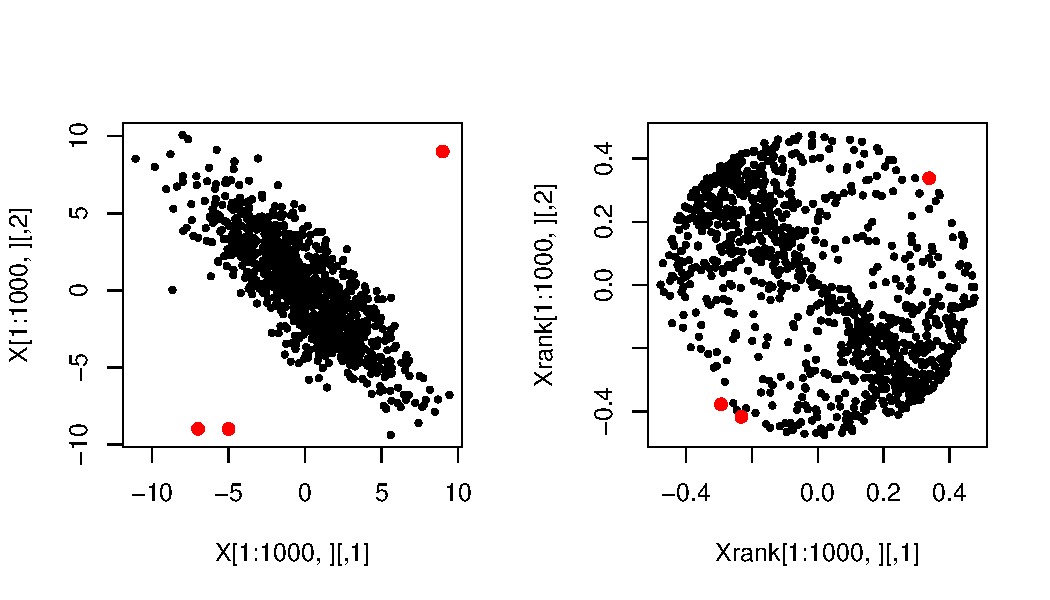
\includegraphics[height=6cm]{../Codes/ranks}
	\caption{(Left) 1000 points randomly drawn from $\mathcal N_2\left((0,0)^T, \left(\protect\begin{smallmatrix} 5 & -4 \\ -4 & 5 \protect\end{smallmatrix}\right)\right) $ and (Right) their signed peripherality functions based on halfspace depth}
	\label{fig:rankplot}
\end{figure}

Our weighted sign vector, which we call the {\it signed peripherality} function, is now defined as the product of the spatial sign and transformed peripherality functions:
%
\begin{align}\label{eqn:rank}
\bfR (\bfx; \bfmu_x, \BF) = \bfS(\bfx, \bfmu_x). \kappa_P( P(\bfx, \BF)),
\end{align}
%
where $\kappa_P: \BR \rightarrow \BR$ is a monotone function. Its purpose is to either downweight or upweight the spatial sign of a point based on its peripherality with respect to a data cloud. As seen in the third panel of Figure~\ref{fig:rankplot}, $\bfR (\bfx; \bfmu_x, \BF)$ maps points {\it inside} a ball of finite radius, thus limiting the influence of outlying points {\it and} preserving the magnitude information of data points. In this paper, we demonstrate certain interesting applications of this multivariate rank transformation in robust statistical inference. Notice that for the trivial choice $P( \bfx; \BF) = \| \bfx - \bfmu_{F} \|$ and $\bfmu_x = \bfmu_F, \kappa_P(x)=x$, we get $\bfR (\bfx; \bfmu_x, \BF) = \bfx$. However, in this paper we illustrate how using the rank-transformed data in place of the original data points or their spatial signs leads to interesting robustness results for other choices of the peripherality functions.

The notion of multivariate ranks goes back to \cite{PuriSenBook}, where they take the vector consisting of marginal univariate ranks as multivariate rank vector. Subsequent definitions of multivariate ranks were proposed by \cite{MottonenOja95,HallinPaindaveine02} and \cite{Chernozhukov14}. Compared to them, the advantages of our signed peripherality function are two-fold: interpretability and flexibility. Firstly, as evident in Figure~\ref{fig:rankplot}, our rank transformation preserves the general shape of the data. In fact, if the map $\| \bfx \| \rightarrow P(\bfx, \BF)$ is one-one (given a fixed $\BF$), then it is possible to get back $\bfx$ from $\bfR (\bfx; \bfmu_x, \BF)$. It also provides an intuitive extension to any spatial sign-based methodology. Secondly, there is considerable scope of generalization within the present framework. Given any general inner product space, the definition of signed peripherality remains the same when euclidean norm is replaced by the norm induced by the inner product. Even within $\BR^p$, it is possible to generalize the ranking function in \eqref{eqn:rank} by adding separate transformations on the sign and peripherality functions to obtain alternate representations of the data in lower or higher dimensional spaces. However, we limit our discussion in this paper to the original formulation in \eqref{eqn:rank}.

In this paper, we assume $\BF$ to be an elliptical distribution. Following \cite{FangEtal90}, elliptical distributions can be formally defined here using their characteristic function:
%
\begin{Definition}
A $p$-dimensional random vector $\bfX$ is said to elliptically distributed if and only if there exist a vector $\bfmu \in \mathbb R^p$, a positive semi-definite matrix $\Omega \equiv \Sigma^{-1} \in \mathbb R^{p \times p}$ and a function $\phi: \mathbb R_+ \rightarrow \mathbb R$ such that the characteristic function $\bft \mapsto \phi_{\bfX - \bfmu} (\bft)$ of $\bfX - \bfmu$ corresponds to $\bft \mapsto \phi (\bft^T \Sigma \bft), \bft \in \mathbb R^p$.
\end{Definition}
%
\noindent The density function of an elliptically distributed random variable takes the form:
%
$$
h(\bfx; \bfmu, \Sigma) = |\Omega|^{1/2} g ((\bfx - \bfmu)^T \Omega (\bfx - \bfmu)),
$$
%
where $g$ is a non-negative scalar-valued density function that is continuous and strictly increasing, and is called the \textit{density generator} of the elliptical distribution. For ease of notation, we denote such a distribution by $\mathcal{E} (\bfmu, \Sigma, g)$.


%{\it signed-peripherality function} $\kappa (\cdot)$. We define this function 
%with three parameters $\mu_{x} \in \cH$, $F \in \cM$ and  
%$\mu_{y} \in \cH$,  argument $x \in \cH$ and range $\cH$. More precisely,
%we use two functions $\kappa_{s} : \cH \rightarrow \cH$, 
%$\kappa_{p} : \cH \rightarrow \cH$ that are respectively 
%composed with the sign transformation and the peripherality function, and 
%then multiplied together to obtain the function
%$\kappa : \cH \times \cH \times \cM \times \cH \times \cH \rightarrow \cH$ 
%defined as 
%\ban 
%\kappa (x; \mu_{x}, F, \mu_{y} ) = k_{s} (S (x; \mu_{x})) k_{p} (P (x; F)) + \mu_{y}. 
%\ean
%Within this very generic framework, we will explore two simple choices. We consider 
%$\kappa_{s} (x) = x$, thus this is fixed to be the identity transformation. The two 
%alternatives we consider for $\kappa_{p}$ are 
%$\kappa_{p} (x) = x$ and $\kappa_{p} (x) = \exp (- x)$, thus one is linearly 
%increasing with $x$ while the other is exponentially decreasing.
%
%
%Notice that if we consider $\mu_{y} = \mu_{F} = \mu_{x}$,  
%$\kappa_{s} (x) = \kappa_{p} (x) = x$, and take the very 
%simple peripherality  function $P( x; F) = || x - \mu_{F} ||$, we have 
%$\kappa (x; \mu_{x}, F, \mu_{y} ) \equiv x$ for all choices of parameters 
%$\mu_{x}, F, \mu_{y}$.  Consequently, under this choice of parameters for the 
%$\kappa$-transformation, analyzing a dataset $\{ X_{1}, \ldots, X_{n} \}$ and 
%its $\kappa$-transformed version 
%$\{ Y_{i} = \kappa (X_{i}; \ldots), \ i = 1, \ldots, n \}$ are equivalent. However,
%in this paper we illustrate how other choices of the peripherality function 
%lead to interesting robustness results. We have deliberately set the location 
%parameters $\mu_{x}, \mu_{F}, \mu_{y}$ to be potentially non-identical, this 
%additional flexibility has some advantage for robust data analysis. In many 
%applications, the value of these three parameters may be identical, which leads 
%to no conflict in our framework.

\paragraph{Organization of paper.}

\paragraph{Notation.}

\section{Weighted sign vectors in location problem}
\label{section:LocSection}
In this section, we focus on the general situation of estimating or testing for the location parameter $\bfmu \equiv \bfmu_F$ using the weighted sign vectors in \eqref{eqn:rank}. We impose the following very general conditions on the weights $w(\bfx, \BF) := \kappa_P(P(\bfx, \BF))$:

\vspace{1em}
\noindent{\bf (A1)} The weights are affine invariant, i.e.
%
$$
w(\bfA \bfx + \bfb, \bfA \BF + \bfb) = w(\bfx, \BF),
$$
%
for any $\bfb \in \BR^p$ and full rank matrix $\bfA \in \BR^{p \times p}$.

\noindent{\bf (A2)} Given a fixed $\BF$, the weights are square-integrable:
%
$$
\int [w(\bfy, \BF)]^2 d\BG(\bfy) < \infty; \BG \in \cM.
$$

\vspace{1em}
\noindent Because of the affine invariance, it is possible to simplify the weight as a function of the norm of $\bfz = \Sigma^{-1/2} (\bfX - \bfmu)$: $w(\bfx, \BF) = f(r)$, with $r = \| \bfz \|$.

A straightforward use of weighted signs in a location problem is to construct an outlier-robust alternative to the Hotelling's $T^2$ test using their sample mean vector and covariance matrix. Formally, this means testing for $H_0: \bfmu = {\bf 0}_p$ vs. $H_1:\bfmu \neq {\bf 0}_p$  based on the test statistic:
%
$$
T_{n,w} = n \bar\bfX_w^T ( \BV \BX_w)^{-1} \bar\bfX_w,
$$
%
({\colrbf define $\BX_w$}) with $\bar\bfX_w = \sum_{i=1}^n \bfX_{w,i}/n$ and $\bfX_{w,i} = w(\bfX_i ) \bfS (\bfX_i)$ for $i=1,2,...,n$. However, the following holds true for this weighted sign test:
%
\begin{Proposition}\label{proposition:SignTest}
Consider $n$ random variables $Z = (\bfZ_1,...,\bfZ_n)^T$ distributed independently and identically as $\mathcal{E}( \bfmu, k \bfI_p, g); k \in \mathbb R$, and the class of hypothesis tests defined above. Then, given any $\alpha \in (0,1)$, local power at $\bfmu \neq {\bf 0}_p$ for the level-$\alpha$ test  based on $T_{n,w}$ is maximum when $w(\bfZ_1) = c$, a constant independent of $\bfZ_1$.
\end{Proposition}
%
\noindent This essentially means that power-wise the (unweighted) spatial sign test \citep{OjaBook10} is optimal in the given class of hypothesis tests when the data comes from a spherically symmetric distribution. Our simulations show that this empirically holds for non-spherical but elliptic distributions as well.

\subsection{The weighted spatial median} 
To explore usage of weighted spatial signs in the location problem that improve upon the state-of-the-art, we concentrate on the following optimization problem:
%
\begin{equation}\label{eqn:WtSpMed}
\bfmu_w = \argmin_{\bfmu_0 \in \mathbb{R}^p} \BE ( w(\bfX) | \bfX - \bfmu_0 |).
\end{equation}
%
This can be seen as a generalization of the Fermat-Weber location problem (which has the spatial median \citep{brown83, Chaudhuri96} as the solution) using data-dependent weights. Using affine equivariant weights in \eqref{eqn:WtSpMed} ensures that the weights are independent of $\bfmu_0$, allowing the optimization problem to have a unique solution. We call this solution the \textit{weighted spatial median} of $\BF$, and denote it by $\bfmu_w$. In a sample setup it is estimated by iteratively solving the equation $\sum_{i=1}^n w(\bfX_i) \bfS (\bfX_i - \hat\bfmu_w)/n = {\bf 0}_p$.

The sample weighted spatial median $\hat\bfmu_w$ is a $\sqrt n$-consistent estimator of $\bfmu_w$, with the following result gives its asymptotic distribution:
%
\begin{Theorem}
Let $\bfA_w, \bfB_w$ be two matrices, dependent on the weight function $w$ such that
%
$$
\bfA_w = \BE \left[ \frac{w( \bfepsilon ) }{\| \bfepsilon \|} \left( 1 - \frac{\bfepsilon \bfepsilon^T}{\| \bfepsilon \|^2} \right) \right];
\quad
\bfB_w = \BE \left[ \frac{(w( \bfepsilon ))^2 \bfepsilon \bfepsilon^T}{\| \bfepsilon \|^2} \right]
$$
%
where $\bfepsilon \sim \mathcal E({\bf 0}, \Sigma, g)$. Then
%
\begin{equation}
\sqrt n (\hat\bfmu_w - \bfmu_w) \leadsto \cN_p ({\bf 0}, \bfA_w^{-1} \bfB_w \bfA_w^{-1})
\end{equation}
\end{Theorem}
%

%We provide a sketch of its proof in the supplementary material, which generalizes equivalent results for the spatial median \citep{OjaBook10}. 
Setting $w(\bfepsilon)=1$ above yields the asymptotic covariance matrix for the spatial median. Following this, the asymptotic relative efficiency (ARE) of $\bfmu_w$ corresponding to some non-uniform weight function with respect to the spatial median, say $\bfmu_s$ will be:
%
$$
ARE( \bfmu_w, \bfmu_s) = \left[ \frac{\text{det} (\bfA^{-1} \bfB \bfA^{-1})}{\text{det} ( \bfA_w^{-1} \bfB_w \bfA_w^{-1})} \right]^{1/p}
$$
%
with $\bfA = \BE [ 1/ \| \bfepsilon \| ( I_p - \bfepsilon \bfepsilon^T/ \| \bfepsilon \|^2 ) ]$ and $\bfB = \BE [ \bfepsilon \bfepsilon^T/ \| \bfepsilon \|^2 ]$. This is further simplified under spherical symmetry:

\begin{Corollary}
For the spherical distribution $\mathcal{E}(\bfmu, k \bfI_p, g); k \in \mathbb R, \bfmu \in \mathbb R^p$, we have
%
$$
ARE( \bfmu_w, \bfmu_s) = \frac{ \left[ \BE \left( \frac{f(r)}{r} \right) \right]^2}{\BE f^2(r) \left[ \BE \left( \frac{1}{r} \right) \right]^2 }
$$
\end{Corollary}
%
\begin{table}[t]
	\centering
    \begin{tabular}{c|ccccc}
    \hline
    & $t_3$   & $t_5$   & $t_{10}$  & $t_{20}$  & Normal \\ \hline
    $p=5$    & 1.28 & 1.20 & 1.16 & 1.14 & 1.13   \\
    $p=10$   & 1.15 & 1.10 & 1.07 & 1.07 & 1.06   \\
    $p=20$   & 1.09 & 1.05 & 1.04 & 1.03 & 1.03   \\
    $p=50$   & 1.05 & 1.02 & 1.01 & 1.01 & 1.01   \\ \hline
    \end{tabular}
    \caption{Table of $ARE(\bfmu_w; \bfmu_s)$ for different spherical distributions}
    \label{table:AREtablewsm}
\end{table}
%
Table \ref{table:AREtablewsm} summarizes the AREs for several families of elliptic distributions, numerically calculated using 10,000 random samples, and taking $f(r) = 1/(1+r)$. It is evident from the table that the weighted spatial median outperforms its unweighted counterpart for all data dimensions and distribution families. While the performance is much better for small values of $p$, weighting the signs seems to have less and less effect as $p$ grows larger. Assuming a first-order autoregressive (AR(1)) covariance structure, i.e. $\sigma_{ij} = \rho^{|i-j|}$ with $ \rho \in (0,1)$, results in largely similar ARE values as those obtained in table \ref{table:AREtablewsm} that assume $\Sigma = \bfI_p$.

\subsection{A high-dimensional test of location}

It is possible to take an alternative approach to the location testing problem by using the covariance-type U-statistic $C_{n,w} = \sum_{i=1}^n \sum_{j=1}^{i-1} \bfX_{w,i}^T \bfX_{w,j}$. This class of test statistics are especially attractive since they are readily generalized to cover high-dimensional situations, i.e. when $p > n$. The Chen and Qin (CQ) high-dimensional test of location for multivariate normal $\bfX_i$ \citep{ChenQin10} is a special case of this test that uses the statistic $C_n = \sum_{i=1}^n \sum_{j=1}^{i-1} \bfX_i^T \bfX_j$. The testing procedure of \cite{WangPengLi15} (from here on referred to as WPL test) shows that one can improve upon the power of the CQ test for non-gaussian elliptical distributions by using spatial signs $\bfS(\bfX_i)$ in place of the actual variables.

Under mild regularity conditions in the lines of \cite{WangPengLi15}, the following results hold for our generalized test statistic $C_{n,w}$ under $H_0$ as $n,p \rightarrow \infty$:
%
\begin{equation}\label{eqn:hdtest1}
\frac{C_{n,w}}{\sqrt{\frac{n(n-1)}{2} \text{Tr}(\bfB_w^2)}} \leadsto N(0,1),
\end{equation}
%
and under contiguous alternatives $H_1: \bfmu = \bfmu_0$,
%
\begin{equation}\label{eqn:hdtest2}
\frac{C_{n,w} - \frac{n(n-1)}{2} \bfmu_0^T \bfA_w^2 \bfmu_0 (1 + o(1)) }{\sqrt{\frac{n(n-1)}{2} \text{Tr}(\bfB_w^2)}} \leadsto N(0,1).
\end{equation}
%
We provide the details behind deriving these two results in the supplementary material, which extend the results of \cite{WangPengLi15} in a weightd sign setup using modified regularity conditions.

Following this, the ARE of this test statistic with respect to its unweighted version, i.e. the WPL statistic, is expressed as:
%
$$
ARE(C_{n,w}, \text{WPL}; \bfmu_0) = \frac{\bfmu_0^T \bfA_w^2 \bfmu_0}{\bfmu_0^T \bfA^2 \bfmu_0} \sqrt\frac{\text{Tr}(\bfB^2)}{\text{Tr}(\bfB_w^2)} (1 + o(1)),
$$
%
when $\Sigma = k \bfI_p$, this again simplifies to $\BE^2(f(r)/r)/[\BE f^2(r). \BE^2(1/r)]$. Thus the ARE values are exactly same as those in Table \ref{table:AREtablewsm}, indicating that for large data dimensions the WPL test and that based on $C_{n,w}$ are almost equivalent.

However, in a practical high-dimensional setup sample sizes are often small. Thus, comparing the the two tests with respect to their \textit{finite sample} efficiencies instead gives a better idea of their practical utility. We do so in table~\ref{table:AREtablehd}, which lists empirical powers calculated from 1000 replications of each setup under an AR(1) covariance structure (with $\rho = 0.8$). While under $H_0: \bfmu = {\bf 0}_p$ all tests have similar performance, $C_{n,w}$ beats the other two under deviations from the null.

\begin{table}
\centering
    \begin{tabular}{cc|ccc}\hline
\multicolumn{5}{l}{$\bfmu = \text{rep}(.15,p)$}\\\hline 
 $p$  & $n$    & CQ   & WPL  & $C_{n,w}$ \\\hline 
  500 & 20 & 0.051 & 0.376 & 0.418 \\
  500 & 50 & 0.060 & 0.832 & 0.866 \\
 1000 & 20 & 0.044 & 0.541 & 0.584 \\
 1000 & 50 & 0.039 & 0.973 & 0.987 \\\hline
\multicolumn{5}{l}{$\bfmu = \text{rep}(0,p)$}\\\hline
 $p$  & $n$    & CQ   & WPL  & $C_{n,w}$ \\\hline 
  500 & 20 & 0.049 & 0.061 & 0.063 \\
  500 & 50 & 0.039 & 0.061 & 0.064 \\
 1000 & 20 & 0.042 & 0.060 & 0.063 \\
 1000 & 50 & 0.043 & 0.050 & 0.050 \\\hline
    \end{tabular}
    \caption{Table of empirical powers of level-0.05 tests for the Chen and Qin (CQ), WPL and $C_{n,w}$ statistics}
    \label{table:AREtablehd}
\end{table}

\section{Inverse depth and estimation of scatter}
\label{section:dcmSection}
We elaborate on the problem estimating the covariance matrix $\Sigma$ and its eigenvectors and eigenvalues using signed peripherality functions in this section. In addition to conditions (P) and (A1), we assume the following conditions on these functions in this section:

\vspace{1em}
\noindent\textbf{(B1)} The following holds:
$$
P(\bfx; \BF) \leq P(\bfmu_F + t(\bfx - \bfmu_F), \BF),
$$
%
for any $\bfx \in \BR^p$ and $t \in (0,1)$.

\noindent\textbf{(B2)} There exists a positive constant $M(P,\BF) $ such that $P(\bfx; \BF) \rightarrow M(P,\BF)$ as $\|\bfx\| \rightarrow \infty $.
\vspace{1em}

Condition (A2) in Section~\ref{section:LocSection} is now replaced by the stronger condition (B2). Note that all the current conditions are essentially the opposite of those imposed on a traditional depth function \citep{zuo00}. Given a depth function, the peripherality functions in this section can be defined as a bounded monotonically decreasing function of it. Consequently, we use the term {\it inverse depth function} in place of peripherality functions in this section, denoting them by $D^-(\bfx,\BF)$, or equivalently $D^-_\bfX(\bfx)$.

Given an inverse depth function $D^-_{\bfX}(\bfx)$ we transform the original random variable as: $\tilde \bfX = D^-_\bfX(\bfx) \bfS(\bfx - \bfmu)$. We attempt to use these vector as the proxy of original data for improved estimation of the components of the population covariance matrix $\Sigma$ in this section. To this end, in Section~\ref{subsec:dcm} we give some results characterizing the population covariance matrix of these vectors, i.e. $\BV \tilde \bfX$, and its affine equivariant counterpart.

%Data depth is as much a property of a vector-valued random variable $\bfX \in \mathbb{R}^p$ as it is of the underlying distribution $F$, so for ease of notation while working with transformed random variables, from now on we shall be using $D_\bfX(\bfx) = D(\bfx, F)$ to denote the depth of a point $\bfx$. Now, given a depth function $D_{\bfX}(\bfx)$ (equivalently, an htped function $D^-_\bfX(\bfx) = D^-(\bfx, F)$), transform the original random variable as: $\tilde \bfx = \tilde D_\bfX(\bfx) \bfS(\bfx - \bfmu)$, $\bfS(.)$ being the spatial sign functional. The transformed random variable $\tilde \bfX$ can be seen as the multivariate rank corresponding to $\bfX$ (e.g. \cite{serfling2006}). 

%Figure \ref{fig:rankplot} gives an idea of how the multivariate rank vector $\tilde \bfX$ is distributed when $\bfX$ has a bivariate normal distribution. Compared to the spatial sign, which are distributed on the surface of $p$-dimensional unit ball centered at $\bfmu$, these spatial ranks have the same direction as original data and reside \textit{inside} the $p$-dimensional ball around $\bfmu$ that has radius $M_D(F)$ (which, for the case of halfspace depth, equals 0.5).

\subsection{Depth Covariance Matrix}
\label{subsec:dcm}
Consider the spectral decomposition of $\Sigma$: $\Sigma = \Gamma\Lambda\Gamma^T$, $\Gamma$ being orthogonal and $\Lambda$ diagonal with positive diagonal elements $\lambda_1, \ldots, \lambda_p$. Also normalize the original random variable as $\bfZ = \Gamma^T\Lambda^{-1/2} (\bfX - \bfmu)$. In this setup, we can represent the transformed random variable as
%
\begin{eqnarray}
\tilde \bfX &=& D^-_{\bfX} (\bfX) \bfS(\bfx - \bfmu) \notag \\
&=& D^-_{\Gamma\Lambda^{1/2}\bfZ + \bfmu} (\Gamma\Lambda^{1/2} \bfZ + \bfmu). \bfS(\Gamma\Lambda^{1/2} \bfZ) \notag \\
&=& \Gamma D^-_{\bfZ}(\bfZ) \bfS(\Lambda^{1/2}\bfZ) \notag \\
&=& \Gamma \Lambda^{1/2} D^-_{\bfZ}(\bfZ) \bfS(\bfZ) \frac{\| \bfZ \|}{\|\Lambda^{1/2} \bfZ \|}.
\label{equation:rankdecomp}
\end{eqnarray}
%
%Because of affine (thus rotational) invariance of a depth function, the depth (htped) value at $\bfz$ does not depend on the direction of $\bfz$, i.e. $D^-_{\bfZ}(\bfz)$ and $\bfS(\bfz)$ are independent. Furthermore,
%$$ Cov \left(\bfS (\bfz), \frac{\| \bfz \|}{\|\Lambda^{1/2} \bfz\|} \right) = E \left(\bfS (\bfz). \frac{\| \bfz \|}{\|\Lambda^{1/2} \bfz\|} \right) - E \bfS (\bfz) E \left(\frac{\| \bfz \|}{\|\Lambda^{1/2} \bfz\|} \right) = E \left( \frac{\bfz}{\|\Lambda^{1/2} \bfz\|} \right) = \bf0$$
%both $\bfS (\bfz)$ and $\bfz / \| \Lambda^{1/2}\bfz \|$ are odd functions of $\bfz$, which has a circularly symmetric distribution, hence each of them has expectation $\bf0$. Consequently, we obtain an expression for the covariance matrix of $\tilde \bfX$:

$D^-_\bfZ(\cdot)$ is an even function in its argument because of affine invariance, as is $\| \bfz \| / \|\Lambda^{1/2} \bfz \|$. Since the sign function $\bfS(\cdot)$ is odd in its argument, it follows that $\BE \tilde \bfX = \bf0$. Consequently, we obtain an expression for $\BV \tilde \bfX$, which we call the {\it Depth Covariance Matrix} (DCM):

\begin{Theorem} \label{Theorem:covform}
Let the random variable $\bfX \in \mathbb{R}^p$ follow an elliptical distribution with center $\bfmu$ and covariance matrix $\Sigma = \Gamma\Lambda\Gamma^T$, its spectral decomposition. Then, given a depth function $D_\bfX(.)$ the covariance matrix of the transformed random variable $\tilde\bfX$ is
\begin{equation} \label{equation:covformEq1}
\BV \tilde \bfX) = \Gamma \Lambda_{D} \Gamma^T,\quad\mbox{with}\quad \Lambda_{D} = \mathbb E_\bfZ \left[ (D^-_\bfZ(\bfz))^2 \frac{\Lambda^{1/2} \bfz \bfz^T \Lambda^{1/2}}{\bfz^T \Lambda \bfz} \right],
\end{equation}
where $\bfZ = (Z_1,...,Z_p)^T \sim N({\bf 0}, \bfI_p)$, so that $\Lambda_{D}$ a diagonal matrix with diagonal entries
%
$$
\lambda_{D,i} = \mathbb E_\bfZ \left[ \frac{(D^-_\bfZ(\bfz))^2 \lambda_i z_i^2}{\sum_{j=1}^p \lambda_j z_j^2} \right].
$$
\end{Theorem}

The matrix of eigenvectors $\Gamma$ remains unchanged in the transformation $\bfX \rightarrow \tilde \bfX$. As a result, the multivariate rank vectors can be used for robust principal component analysis, which we are going to discuss shortly. However, as one can see in the above expression, the diagonal entries of $\Lambda_{D}$ do not change if a scale change is done on all entries of $\Lambda$, meaning the $\Lambda_{D}$ matrices corresponding to $\BF$ and $c \BF$ for some $c \neq 0$ will be same. This is the reason the DCM is not equivariant under affine transformations.

We need to follow the general framework of M-estimation with data-dependent weights \citep{HuberBook81} to construct an affine equivariant counterpart of the DCM. Specifically, we implicitly define the Affine-equivariant Depth Covariance Matrix (ADCM) as
%
\begin{equation} \label{eqn:ADCM}
\Sigma_{Dw} = \frac{1}{ \BV \tilde Z_1 } \BE_\bfX \left[ \frac{(D^-_\bfX(\bfx))^2 (\bfx - \bfmu) (\bfx - \bfmu)^T}{(\bfx - \bfmu)^T \Sigma_{Dw}^{-1} (\bfx - \bfmu)} \right].
\end{equation}
%
Its affine equivariance follows from the fact that the weights $(D^-_\bfX (\bfx))^2$ depend only on the standardized quantities $\bfz \sim \cE ({\bf 0}, k \bfI_p, g)$. We solve (\ref{eqn:ADCM}) iteratively by obtaining a sequence of positive definite matrices $\Sigma^{(k)}_{Dw}$ until convergence:
%
$$
\Sigma^{(k+1)}_{Dw} = \frac{1}{\BV \tilde Z_1 } \BE_\bfX \left[ \frac{(D^-_\bfX(\bfx))^2 (\Sigma^{(k)}_{Dw})^{1/2} (\bfx - \bfmu) (\bfx - \bfmu)^T (\Sigma^{(k)}_{Dw})^{1/2}}{(\bfx - \bfmu)^T (\Sigma^{(k)}_{Dw})^{-1} (\bfx - \bfmu)} \right].
$$
%

To ensure existence and uniqueness of this estimator, let us consider the class of scatter estimators $\Sigma_M$ that are obtained as solutions of the following equation:
%
\begin{equation}
E_{\bfZ_M} \left[ u( \| \bfz_M \| )  \frac{\bfz_M \bfz_M^T}{\| \bfz_M \|^2}  - v( \| \bfz_M \| ) I_p \right] = 0
\end{equation}
%
with $\bfz_M = \Sigma_M^{-1/2} (\bfx - \bfmu)$. Under the following assumptions on the scalar valued functions $u$ and $v$, the above equation produces a unique solution \citep{HuberBook81}:
%

\vspace{1em}
\noindent\textbf{(M1)} The function $u(r)/r^2$ is monotone decreasing, and $u(r)>0$ for $r>0$;

\noindent\textbf{(M2)}  The function $v(r)$ is monotone decreasing, and $v(r)>0$ for $r>0$;

\noindent\textbf{(M3)} Both $u(r)$ and $v(r)$ are bounded and continuous;

\noindent\textbf{(M4)} $u(0) / v(0) < p$;

\noindent\textbf{(M5)} For any hyperplane in the sample space $\mathcal X$, (i) $P(H) = E_\bfX 1_{\bfx \in H} < 1 - p v(\infty) / u(\infty)$ and (ii) $P(H) \leq 1/p$.
%

\vspace{1em}
\noindent In our case we take $v(r) = Var(\tilde Z_1)$, i.e. a constant, thus (M2) and (M3) are trivially satisfied. As for $u$, we notice that most well-known depth functions can be expressed as simple functions of the norm of the standardized random variable. For example, $PD_\bfZ (\bfz) = (1 - G(\| \bfz \|); MhD_\bfZ (\bfz) = (1+\| \bfz \|^2)^{-1}; HSD_\bfZ (\bfz) = (1+\| \bfz \|)^{-1}$ etc., so that we can take as $u$ square of the corresponding peripherality functions:
% Var(Z1) breaks into two independent parts: depth and sign. So can check m4 and M5 here itself.
$$
u_{PD} (r) = G^2 (r); \quad u_{MhD}(r)  = \frac{r^4}{(1 + r^2)^2}; \quad u_{HSD}(r)  = \frac{r^2}{(1 + r/G^{-1}(0.75))^2}
$$
%

It is easy to verify that the above choices of $u$ satisfy (M1) and (M3). To check (M4) and (M5), first notice that $\bfZ$ has a spherically symmetric distribution, so that its norm and sign are independent. Since $D_\bfZ(\bfz)$ depends only on $\| \bfz \|$, we have
%
$$
Var (\tilde Z_1) = Var \left( D^-_\bfZ (\bfZ) \frac{Z_1}{ \|\bfZ \|} \right) = Var (D^-_\bfZ (\bfZ)) Var (S_1 (\bfZ)) = \frac{1}{p} Var (D^-_\bfZ (\bfZ))
$$
%
as $Cov(\bfS(\bfZ)) = Cov((S_1(\bfZ), S_2(\bfZ), ..., S_p(\bfZ))^T) = I_p/p$. Now for MhD and HSD $u(\infty)=1, u(0)=0$, so (M4) and (M5) are immediate. To achieve this for PD, we only need to replace $u_{PD}(r)$ with $u_{PD}^*(r) = G^2(r) - 1/4$.

\subsection{Calculating the sample DCM and ADCM}
Let us now consider $n$ iid random draws from our elliptic distribution $F$, say $\bfX_1,...,\bfX_n$. For ease of notation, denote $SS(\bfx; \bfmu) = \bfS(\bfx - \bfmu) \bfS(\bfx - \bfmu)^T$. Then, given the depth function and known location center $\bfmu$, one can show that the vectorized form of $\sqrt n$-times the sample DCM: $\sum_{i=1}^n (D^-_\bfX(\bfx_i))^2SS(\bfx_i; \bfmu) /\sqrt{n}$  has an asymptotic multivariate normal distribution with mean $\sqrt n.vec(E[( (D^-_\bfX (\bfX))^2 SS(\bfx; \bfmu)])$ and a certain covariance matrix by straightforward application of the central limit theorem (CLT). But in practice the population depth function $D_\bfX(\bfx) = D(\bfx, F)$ is estimated by the depth function based on the empirical distribution function, $F_n$. Denote this sample depth by $D^n_\bfX (\bfx) = D(\bfx, F_n)$. Here we make the following assumption regarding how it approximates $D_\bfX(\bfx)$:

\vspace{1em}
\noindent\textbf{(D5)} \textit{Uniform convergence}: $\sup_{\bfx \in \mathbb R^p} | D^n_\bfX (\bfx) - D_\bfX (\bfx) | \rightarrow 0$ as $n \rightarrow \infty $.
\vspace{1em}

The assumption that empirical depths converge uniformly at all points $\bfx$ to their population versions holds under very mild conditions for several well known depth functions: for example projection depth \citep{zuo03} and simplicial depth \citep{Dumbgen92}. One also needs to replace the known location parameter $\bfmu$ by some estimator $\hat\bfmu_n$. Examples of robust estimators of location that are relevant here include the spatial median \citep{haldane48,brown83}, Oja median \citep{oja83}, projection median \citep{zuo03} etc. Now, given $D^n_\bfX(.)$ and $\hat \bfmu_n$, to plug them into the sample DCM and still go through with the CLT we need the following result:

\begin{Lemma} \label{Lemma:lemma1}
Consider a random variable $\bfX \in \mathbb{R}^p$ having a continuous and symmetric distribution with location center $\bfmu$ such that $E\|\bfx - \bfmu \|^{-3/2} < \infty$. Given $n$ random samples from this distribution, suppose $\hat\bfmu_n$ is an estimator of $\bfmu$ so that $\sqrt n (\hat\bfmu_n - \bfmu) = O_P(1) $. Then with the above notations, and given the assumption (D5) we have
%
$$ \sqrt n \left[
\frac{1}{n} \sum_{i=1}^n (D^{-n}_\bfX (\bfx_i))^2 SS(\bfx_i; \hat\bfmu_n) -
\frac{1}{n} \sum_{i=1}^n (D^-_\bfX (\bfx_i))^2 SS(\bfx_i; \bfmu) \right]
\stackrel{P}{\rightarrow} 0 $$
\end{Lemma}

Following this, we are now in a position to state the result for consistency of the sample DCM:

\begin{Theorem} \label{Theorem:rootn}
Consider $n$ iid samples from the distribution in Lemma \ref{Lemma:lemma1}. Then, given a depth function $D_\bfX(.)$ and an estimate of center $\hat\bfmu_n$ so that $\sqrt n(\hat \bfmu_n - \bfmu) = O_P(1)$,
%
$$ \sqrt n \left[ vec\left\{ \frac{1}{n} \sum_{i=1}^n (D^{-n}_\bfX (\bfx_i))^2 SS(\bfx_i; \hat\bfmu_n) \right\} - E \left[ vec\left\{ (D^-_\bfX (\bfx))^2 SS(\bfx; \bfmu) \right\} \right] \right]
\stackrel{D}{\rightarrow}
N_{p^2} ({\bf 0}, V_{D,S}(F)) $$
$$ \text{with } V_{D,S}(F) = Var \left[vec \left\{ (D^-_\bfX (\bfx))^2 SS(\bfx; \bfmu) \right\} \right] $$
\end{Theorem}

\noindent In case $F$ is elliptical, an elaborate form of the covariance matrix $V_{D,S}(F)$ explicitly specifying each of its elements (more directly those of its $\Gamma^T$-rotated version) can be obtained, which is given in Appendix \ref{section:appA}. This form is useful when deriving limiting distributions of eigenvectors and eigenvalues of the sample DCM.

In contrast to the DCM, the issue of estimating $\bfmu$ to plug into the ADCM is easily handled by simultaneously solving for the location and scatter functionals ($\bfmu_{Dw}, \Sigma_{Dw}$):
%
\begin{eqnarray}
E \left[ \frac{\Sigma_{Dw}^{-1/2} (\bfx - \bfmu_{Dw})}{ \| \Sigma_{Dw}^{-1/2}(\bfx - \bfmu_{Dw}) \|} \right] &=& {\bf 0}_p \label{eqn:AffineMedian}\\
E \left[ \frac{(D^-_\bfX(\bfx))^2 \Sigma_{Dw}^{-1/2} (\bfx - \bfmu_{Dw}) (\bfx - \bfmu_{Dw})^T \Sigma_{Dw}^{-1/2}}{(\bfx - \bfmu_{Dw})^T \Sigma_{Dw}^{-1} (\bfx - \bfmu_{Dw})} \right] &=& Var (\tilde Z_1) I_p \label{eqn:AffineCov}
\end{eqnarray}
%
In the framework of (\ref{eqn:ADCM}), for any fixed $\Sigma_M$ there exists a unique and fixed solution of the location problem $E_{\bfZ_M} (w(\| \bfz_M \| \bfz_M) = {\bf 0}_p $ under the following condition:

\vspace{1em}
\noindent\textbf{(M6)} The function $w(r)r$ is monotone increasing for $r>0$.

\vspace{1em}
\noindent This condition is easy to verify for our choice of the weights: $w(\| \bfz_M \| ) = D^-_{\bfZ_M} (\bfz_M) / \| \bfz_M \|$. Uniqueness of simultaneous fixed point solutions of \ref{eqn:AffineMedian} and \ref{eqn:AffineCov} is guaranteed when $\bfX$ has a symmetric distribution \citep{HuberBook81}.

In practice it is difficult to calculate the scale multiple $Var (\tilde Z_1)$ analytically for known depth functions and an arbitrary $F$. Here we instead obtain its standardized version $\Sigma_{Dw}^* = \Sigma_{Dw} / Var(\tilde Z_1)$ (so that the determinant equals 1), alongwith $\bfmu_{Dw}$ using the following iterative algorithm:

\begin{enumerate}
\item Start from some initial estimates $(\bfmu_{Dw}^{(0)}, \Sigma_{Dw,(0)})$. Set $t=0$;

\item Calculate the standardized observations $\bfz_i^{(t)} = \Sigma_{Dw,(t)}^{-1/2} (\bfx_i - \bfmu_{Dw}^{(t)})$;

\item Update the location estimate:
%
$$
\bfmu_{Dw}^{(t+1)} = \frac{\sum_{i=1}^n \tilde \bfx_i / \| \bfz_i^{(t)} \| }{\sum_{i=1}^n 1 / \| \bfz_i^{(t)} \|}
$$
%
\item Update the scatter estimate:
%
$$
\Sigma_{Dw}^{*(t+1)} = \frac{1}{n} \sum_{i=1}^n \frac{(D^{-n}_\bfX (\bfx_i))^2 (\bfx_i - \bfmu_{Dw}^{(t+1)})(\bfx_i - \bfmu_{Dw}^{(t+1)})^T}{\| \bfz_i^{(t)} \|^2}; \quad \Sigma_{Dw}^{*(t+1)} \leftarrow \frac{\Sigma_{Dw}^{*(t+1)}}{\text{det} (\Sigma_{Dw}^{*(t+1)})^{1/p}}
$$
%
\item Continue until convergence.
\end{enumerate}

\subsection{Robust PCA using eigenvectors}

Since we are mainly interested in using the DCM for robust principal components analysis, from now on we assume that the eigenvalues of $\Sigma$ are distinct: $\lambda_1 > \lambda_2 > ... > \lambda_p$ to obtain asymptotic distributions of its eigenvectors. In case any of the eigenvalues have multiplicity larger than 1, limiting distributions of the corresponding eigenprojection matrices can be obtained analogous to those of the sign covariance matrix \citep{magyar14}.

\subsubsection{Influence functions}
We start with deriving the influence functions for eigenvectors of the DCM and ADCM. This will help in demonstrating the robustness of their estimates, as well as deriving the asymptotic distributions of their sample counterparts. Influence functions of the DCM as well as its eigenvectors and eigenvalues, which are essential to understand how much influence a sample point, especially an infinitesimal contamination, has on any functional on the distribution \citep{HampelBook86}. Given any probability distribution $F$, the influence function of any point $\bfx_0$ in the sample space $\mathcal{X}$ for some functional $T(F)$ on the distribution is defined as
%
$$ IF(\bfx_0; T,F) = \lim_{\epsilon \rightarrow 0} \frac{1}{\epsilon} (T(F_\epsilon) - T(F)) $$
%
where $F_\epsilon$ is $F$ with an additional mass of $\epsilon$ at $\bfx_0$, i.e. $F_\epsilon = (1-\epsilon)F + \epsilon \Delta_{\bfx_0}$; $\Delta_{\bfx_0}$ being the distribution with point mass at $\bfx_0$. When $T(F) = E_F g$ for some $F$-integrable function $g$, $IF(\bfx_0; T,F) = g(\bfx_0) - T(F)$. It now follows that for the DCM,
%
$$ IF(\bfx_0; Cov(\tilde \bfX), F) = (D^-_\bfX(\bfx_0))^2 SS(\bfx_0; \bfmu) - Cov(\tilde \bfX) $$

Following \cite{croux00}, we now get the influence function of the $i^\text{th}$ eigenvector of $Cov(\tilde\bfX)$, say $\bfgamma_D = (\bfgamma_{D,1},...,\bfgamma_{D,p}); i = 1,...,p$:
%
\begin{eqnarray}
IF(\bfx_0; \bfgamma_{D,i}, F) &=& \sum_{k=1; k \neq i}^p \frac{1}{\lambda_{D,S,i} - \lambda_{D,S,k}} \left\{ \bfgamma^T_k IF(\bfx_0; Cov(\tilde \bfX), \bfgamma_i) \right\} \bfgamma_k \notag \\
&=& \sum_{k=1; k \neq i}^p \frac{1}{\lambda_{D,S,i} - \lambda_{D,S,k}} \left\{ \bfgamma^T_k (D^-_\bfX(\bfx_0))^2 SS(\bfx_0; \bfmu)\bfgamma_i - \lambda_{D,S,i}\bfgamma_k^T\bfgamma_i \right\} \bfgamma_k \notag \\
&=& \sum_{k=1; k \neq i}^p \frac{\sqrt{\lambda_i \lambda_k} z_{0i} z_{0k}}{\lambda_{D,S,i} - \lambda_{D,S,k}}. \frac{(D^-_\bfZ(\bfz_0))^2 }{\bfz_0^T \Lambda \bfz_0} \bfgamma_k
\end{eqnarray}
%
where $\Gamma^T \Lambda^{-1/2} (\bfx_0 - \bfmu) = \bfz_0 = (z_{01},...,z_{0p})^T$. Clearly this influence function will be bounded, which indicates good robustness properties of principal components.

For the ADCM, we first notice that the influence function of any affine equivariant estimate of scatter can be expressed as
%
$$
IF(\bfx_0, C, F) = \alpha_C (\| \bfz_0 \| ) \frac{\bfz_0 \bfz_0^T}{\bfz_0^T \bfz_0} - \beta_C( \| \bfz_0 \| ) C
$$
%
for scalar valued functions $\alpha_C, \beta_C$ \citep{HampelBook86}. Following this, the influence function of an eigenvector $\bfgamma_{C,i}$ of $C$ is derived:
%
$$
IF(\bfx_0, \bfgamma_{C,i}, F) = \alpha_C(\| \bfz_0 \|) \sum_{k=1, k \neq i}^p \frac{\sqrt {\lambda_i \lambda_k}}{\lambda_i - \lambda_k}. \frac{z_{0i} z_{0k}}{\bfz_0^T \bfz_0} \bfgamma_k
$$
%
When $C=\Sigma_M$, i.e. the solution to (\ref{eqn:ADCM}), then \cite{HuberBook81} shows that
%
$$
\alpha_C (\| \bfz_0 \|) = \frac{p(p+2) u (\| \bfz_0 \|)}{E_{F_0} \left[ p u(\| \bfy \| ) + u'(\| \bfy \|) \| \bfy \| \right] }
$$
%
Setting $u( \| \bfz_0 \|) = ( D^-_\bfZ (\bfz_0))^2$ ensures that the influence function of eigenvectors of the ADCM is bounded as well as increasing in magnitude with $\| \bfz_0 \|$.

\begin{figure}[]
	\centering
		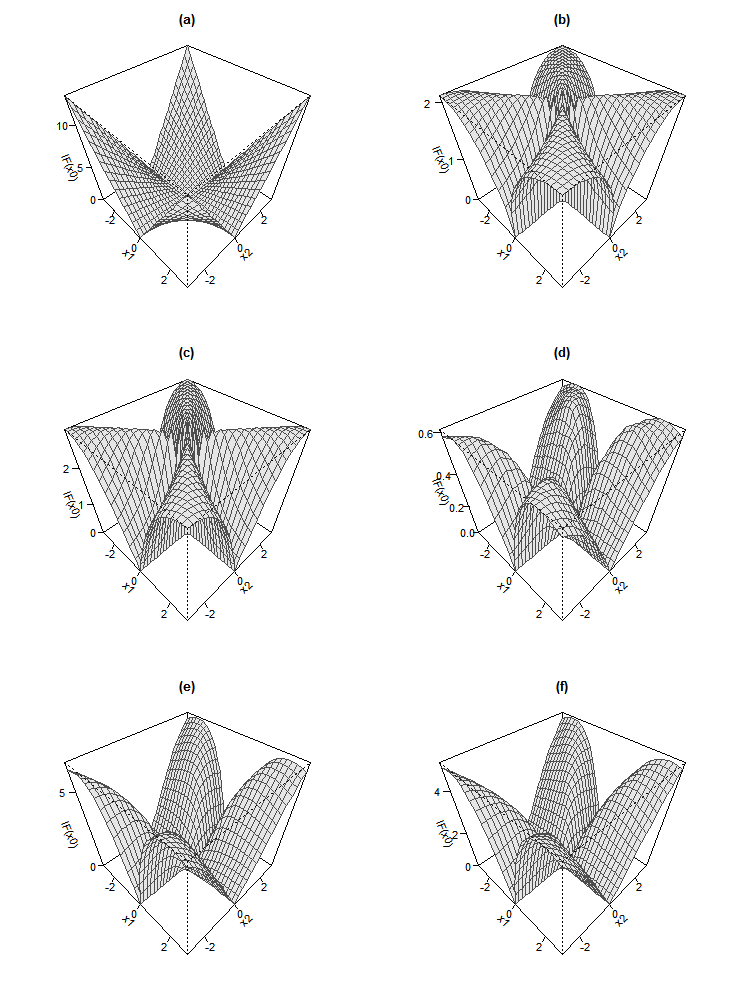
\includegraphics[width=12cm]{../Codes/IFnorm.png}
	\caption{Plot of the norm of influence function for first eigenvector of (a) sample covariance matrix, (b) SCM, (c) Tyler's scatter matrix and DCMs for (d) Halfspace depth, (e) Mahalanobis depth, (f) Projection depth for a bivariate normal distribution with $\bfmu = {\bf 0}, \Sigma = \diag(2,1)$}
	\label{fig:IFnorm}
\end{figure}

In Figure \ref{fig:IFnorm} we consider first eigenvectors of our scatter estimates, as well as teo well-known robust estimates of scatter: the Sign Covariance Matrix (SCM) and Tyler's shape matrix, for the $\mathcal{N}_2((0,0)^T, \diag(2,1))$ and plot norms of these influence functions for different values of $\bfx_0$. Influence function for the $i^\text{th}$ eigenvectors of these two matrices (say $\bfgamma_{S,i}$ and $\bfgamma_{T,i}$, respectively) are as follows:
%
\begin{eqnarray*}
\quad IF(\bfx_0; \bfgamma_{S,i}, F) &=& \sum_{k=1; k \neq i}^p \frac{\sqrt{\lambda_i \lambda_k}}{\lambda_{S,i} - \lambda_{S,k}}. \frac{z_{0i} z_{0k}}{\bfz_0^T \Lambda \bfz_0} \bfgamma_k, \text{ with } \lambda_{S,i} = E_\bfZ \left( \frac{\lambda_i z_i^2}{\sum_{j=1}^p \lambda_j z_j^2} \right) \quad \\
IF(\bfx_0; \bfgamma_{T,i}, F) &=& (p+2) \sum_{k=1; k \neq i}^p \frac{\sqrt{\lambda_i \lambda_k}}{\lambda_i - \lambda_k}. \frac{z_{0i} z_{0k}}{\bfz_0^T \bfz_0} \bfgamma_k \quad 
\end{eqnarray*}
%
Their corresponding plots demonstrate the 'inlier effect', i.e. points close to symmetry center and the center itself having high influence, which results in loss of efficiency. The influence function for the sample covariance matrix is obtained by replacing $(p+2)$ by $\| \bfz_0 \|^2$ in the expression of $IF(\bfx_0; \bfgamma_{T,i}, F)$ above, hence is unbounded and the corresponding eigenvector estimators are not robust. In comparison, all three DCMs considered here have a bounded influence function as well as small values of the influence function at 'deep' points.

\subsubsection{Asymptotic and finite-sample efficiencies}

%Unlike affine equivariant estimators of shape, the Asymptotic Relative Efficiency (ARE) of eigenvectors (with respect to any other affine equivariant estimator) can not be simplified as a ratio of two scalar quantities dependent on only the distribution of $\| \bfz \|$ (e.g. \cite{taskinen12,ollilia03}).
Suppose $\hat C$ is a $\sqrt n$-consistent estimator of a scatter functional $C$. Then the asymptotic variance of its eigenvectors are \cite{anderson}
%
\begin{equation} \label{equation:covevEq}
AVar(\sqrt n\hat \bfgamma_{c,i}) = \sum_{k=1; k \neq i}^p \frac{\lambda_i \lambda_k}{(\lambda_i - \lambda_k)^2} \bfgamma_k \bfgamma_k^T
\end{equation}
%
The asymptotic relative efficiencies of eigenvectors from the sample DCM with respect to the sample covariance matrix can now be derived using (\ref{equation:covevEq}) above and (\ref{equation:DevEq}) from Corollary \ref{Corollary:eigendist}:
%
\begin{eqnarray*}
ARE(\hat\bfgamma^D_i, \hat\bfgamma_i; F) &=& \frac{\Tr( AVar(\sqrt n\hat \bfgamma_i))}{\Tr( AVar(\sqrt n\hat \bfgamma^D_i))}\\
&=& \left[\sum_{k=1; k \neq i}^p \frac{\lambda_i \lambda_k}{(\lambda_i - \lambda_k)^2} \right] \left[ \sum_{k=1; k \neq i}^p \frac{\lambda_i \lambda_k }{(\lambda_{D,s,i} - \lambda_{D,S,k})^2} E \left( \frac{(D^-_\bfZ (\bfz))^4 z_i^2 z_k^2}{(\bfz^T \Lambda \bfz)^2} \right) \right]^{-1}
\end{eqnarray*}

Obtaining ARE of the ADCM is, in comparison to DCM, more straightforward. The asymptotic covariance matrix of an eigenvector of the affine equivariant scatter functional $C$ is given by:
%
$$
AVar (\sqrt n  \hat\bfgamma_{C,j}) = ASV (C_{12}, F_0) \sum_{k=1, k \neq i}^p \frac{\lambda_i \lambda_k}{\lambda_i - \lambda_k}. \bfgamma_i \bfgamma_k^T
$$
%
where $ASV (C_{12}, F_0)$ is the asymptotic variance of an off-diagonal element of $C$ when the underlying distribution is $F_0$. Following \cite{croux00} this equals
%
$$
ASV (C_{12}, F_0) = E_{F_0} \left[ \alpha_c (\| \bfz \|)^2 (S_1(\bfz)S_2 (\bfz))^2 \right] = E_{F_0} \alpha_C (\| \bfz \|)^2 . E_{F_0} (S_1(\bfz)S_2 (\bfz))^2 
$$
% 
again using the fact that $\|\bfZ\|$ and $\bfS(\bfZ)$ are independent with $\bfZ \sim F_0$. It now follows that
%
\begin{equation}
ARE (\hat\bfgamma_{\Sigma_M,i}, \hat\bfgamma_{Cov,i}; F) = \frac{E_{F_0} \alpha_{Cov} (\| \bfz \|)^2}{E_{F_0} \alpha_C (\| \bfz \|)^2} = \frac{E_{F_0} \| \bfz \|^4. \left[ E_{F_0} ( p u \| \bfz\| + u'( \| \bfz \|) \| \bfz \| ) \right]^2}{E_{F_0} (u(\| \bfz \|))^2}
\end{equation}
%

Table \ref{table:AREtable} considers 6 different elliptic distributions (namely, bivariate $t$ with df = 5, 6, 10, 15, 25 and bivariate normal) and summarizes ARE for first eigenvectors for ADCMs corresponding to projection depth (PD-ACM) and halfspace depth (HSD-ACM). Due to difficulty of analytically obtain the AREs, we calculate them using Monte-Carlo simulation of $10^6$ samples and subsequent numerical integration. The ADCM seems to be particularly efficient in lower dimensions for distributions with heavier tails ($t_5$ and $t_6$), while for distributions with lighter tails, the AREs increase with data dimension. At higher values of $p$ the ADCM is almost as efficient as the sample covarnace matrix when the data comes from multivariate normal distribution.

\begin{table}[t]
\centering
    \begin{tabular}{c|cccc|cccc}
    \hline
    & \multicolumn{4}{c|}{PD-ACM} & \multicolumn{4}{c}{HSD-ACM} \\\cline{2-9}
    Distribution & $p=2$  & $p=5$  & $p=10$ & $p=20$ & $p=2$  & $p=5$  & $p=10$ & $p=20$ \\ \hline
    $t_5$           & 4.73 & 3.99 & 3.46 & 3.26 & 4.18 & 3.63 & 3.36 & 3.15 \\
    $t_6$           & 2.97 & 3.28 & 2.49 & 2.36 & 2.59 & 2.45 & 2.37 & 2.32 \\
    $t_{10}$          & 1.45 & 1.47 & 1.49 & 1.52 & 1.30 & 1.37 & 1.43 & 1.49 \\
    $t_{15}$          & 1.15 & 1.19 & 1.23 & 1.27 & 1.01 & 1.10 & 1.17 & 1.24 \\
    $t_{25}$          & 0.97 & 1.02 & 1.07 & 1.11 & 0.85 & 0.94 & 1.02 & 1.08 \\
    MVN          & 0.77 & 0.84 & 0.89 & 0.93 & 0.68 & 0.77 & 0.84 & 0.91 \\ \hline
    \end{tabular}
    \caption{Table of AREs of the ADCM for different choices of $p$ and data-generating distributions, and two choices of depth functions}
    \label{table:AREtable}
\end{table}

We now obtain finite sample efficiencies of the three DCMs as well as their depth-weighted affine equivariant counterparts by a simulation study, and compare them with the same from the SCM and Tyler's scatter matrix. We consider the same 6 elliptical distributions considered in ARE calculations above, and from every distribution draw 10000 samples each for sample sizes $n = 20, 50, 100, 300, 500$. All distributions are centered at ${\bf 0}_p$, and have covariance matrix $\Sigma = \diag(p,p-1,...1)$. We consider 3 choices of $p$: 2, 3 and 4.

We use the concept of principal angles \citep{miao92} to find out error estimates for the first eigenvector of a scatter matrix. In our case, the first eigenvector will be
%
$$ \bfgamma_1 = (1,\overbrace{0,...,0}^{p-1})^T $$
%
For an estimate of the eigenvector, say $\hat\bfgamma_1$, error in prediction is measured by the smallest angle between the two lines, i.e. $ \cos^{-1} | \hat\bfgamma_1^T \hat\bfgamma_1 | $. A smaller absolute value of this angle is equivalent to better prediction. We repeat this 10000 times and calculate the \textbf{Mean Squared Prediction Angle}:
%
$$ MSPA(\hat \bfgamma_1) = \frac{1}{10000} \sum_{m=1}^{10000} \left( \cos^{-1} \left|\bfgamma_1^T \hat\bfgamma^{(m)}_1 \right| \right)^2 $$
%
Finally, the finite sample efficiency of some eigenvector estimate $\hat\bfgamma^E_1$ relative to that obtained from the sample covariance matrix, say $\hat\bfgamma^{Cov}_1$ is obtained as:
$$ FSE(\hat\bfgamma^E_1, \hat\bfgamma^{Cov}_1) = \frac{MSPA(\hat\bfgamma^{Cov}_1)}{MSPA(\hat\bfgamma^E_1)} $$

Tables \ref{table:FSEtable2}, \ref{table:FSEtable3} and \ref{table:FSEtable4} give FSE values for $p=2,3,4$, respectively. In general, all the efficiencies increase as the dimension $p$ goes up. DCM-based estimators (columns 3-5 in each table) outperform SCM and Tyler's scatter matrix, and among the 3 depths considered, projection depth seems to give the best results. Its finite sample performances are better than Tyler's and Huber's M-estimators of scatter as well as their symmetrized counterparts (see Table 4 in \cite{sirkia07}, and quite close to the affine equivariant spatial sign covariance matrix (see Table 2 in \cite{ollilia03}). The depth-weighted iterated versions of these 3 SCMs (columns 6-8 in each table) seem to further better the performance of their corresponding orthogonal equivariant counterparts.

\begin{table}[b]
\begin{footnotesize}
    \begin{tabular}{c|cc|ccc|ccc}
    \hline
    $F$ = Bivariate $t_5$    & SCM  & Tyler & HSD-CM & MhD-CM & PD-CM & HSD-wCM & MhD-wCM & PD-wCM \\ \hline
    $n$=20                   & 0.80 & 0.83  & 0.95   & 0.95   & 0.89  & 1.00    & 0.96    & 0.89   \\
    $n$=50                   & 0.86 & 0.90  & 1.25   & 1.10   & 1.21  & 1.32    & 1.13    & 1.25   \\
    $n$=100                  & 1.02 & 1.04  & 1.58   & 1.20   & 1.54  & 1.67    & 1.24    & 1.63   \\
    $n$=300                  & 1.24 & 1.28  & 1.81   & 1.36   & 1.82  & 1.93    & 1.44    & 1.95   \\
    $n$=500                  & 1.25 & 1.29  & 1.80   & 1.33   & 1.84  & 1.91    & 1.39    & 1.97   \\ \hline
    $F$ = Bivariate $t_6$    & SCM  & Tyler & HSD-CM & MhD-CM & PD-CM & HSD-wCM & MhD-wCM & PD-wCM \\ \hline
    $n$=20                   & 0.77 & 0.79  & 0.92   & 0.92   & 0.86  & 0.96    & 0.92    & 0.85   \\
    $n$=50                   & 0.76 & 0.78  & 1.11   & 1.00   & 1.08  & 1.17    & 1.03    & 1.13   \\
    $n$=100                  & 0.78 & 0.79  & 1.27   & 1.06   & 1.33  & 1.35    & 1.11    & 1.41   \\
    $n$=300                  & 0.88 & 0.91  & 1.29   & 1.09   & 1.35  & 1.38    & 1.15    & 1.45   \\
    $n$=500                  & 0.93 & 0.96  & 1.37   & 1.13   & 1.40  & 1.44    & 1.19    & 1.48   \\ \hline
    $F$ = Bivariate $t_{10}$ & SCM  & Tyler & HSD-CM & MhD-CM & PD-CM & HSD-wCM & MhD-wCM & PD-wCM \\ \hline
    $n$=20                   & 0.70 & 0.72  & 0.83   & 0.84   & 0.77  & 0.89    & 0.87    & 0.79   \\
    $n$=50                   & 0.58 & 0.60  & 0.90   & 0.84   & 0.86  & 0.95    & 0.88    & 0.91   \\
    $n$=100                  & 0.57 & 0.59  & 0.92   & 0.87   & 0.97  & 0.98    & 0.90    & 1.03   \\
    $n$=300                  & 0.62 & 0.64  & 0.93   & 0.85   & 0.99  & 0.99    & 0.91    & 1.06   \\
    $n$=500                  & 0.62 & 0.65  & 0.93   & 0.86   & 1.00  & 1.00    & 0.92    & 1.08   \\ \hline
    $F$ = Bivariate $t_{15}$ & SCM  & Tyler & HSD-CM & MhD-CM & PD-CM & HSD-wCM & MhD-wCM & PD-wCM \\ \hline
    $n$=20                   & 0.63 & 0.66  & 0.76   & 0.78   & 0.72  & 0.81    & 0.81    & 0.73   \\
    $n$=50                   & 0.52 & 0.52  & 0.79   & 0.75   & 0.80  & 0.84    & 0.79    & 0.85   \\
    $n$=100                  & 0.51 & 0.52  & 0.83   & 0.77   & 0.88  & 0.88    & 0.81    & 0.94   \\
    $n$=300                  & 0.55 & 0.56  & 0.84   & 0.79   & 0.91  & 0.89    & 0.84    & 0.98   \\
    $n$=500                  & 0.56 & 0.59  & 0.85   & 0.80   & 0.93  & 0.91    & 0.86    & 0.99   \\ \hline
    $F$ = Bivariate $t_{25}$ & SCM  & Tyler & HSD-CM & MhD-CM & PD-CM & HSD-wCM & MhD-wCM & PD-wCM \\ \hline
    $n$=20                   & 0.63 & 0.65  & 0.77   & 0.79   & 0.74  & 0.80    & 0.81    & 0.74   \\
    $n$=50                   & 0.49 & 0.50  & 0.73   & 0.71   & 0.76  & 0.78    & 0.75    & 0.80   \\
    $n$=100                  & 0.45 & 0.46  & 0.73   & 0.69   & 0.81  & 0.78    & 0.73    & 0.87   \\
    $n$=300                  & 0.51 & 0.52  & 0.78   & 0.75   & 0.87  & 0.83    & 0.79    & 0.94   \\
    $n$=500                  & 0.53 & 0.55  & 0.79   & 0.75   & 0.87  & 0.84    & 0.80    & 0.94   \\ \hline
    $F$ = BVN                & SCM  & Tyler & HSD-CM & MhD-CM & PD-CM & HSD-wCM & MhD-wCM & PD-wCM \\ \hline
    $n$=20                   & 0.56 & 0.60  & 0.69   & 0.71   & 0.67  & 0.73    & 0.74    & 0.68   \\
    $n$=50                   & 0.42 & 0.43  & 0.66   & 0.66   & 0.70  & 0.71    & 0.69    & 0.75   \\
    $n$=100                  & 0.42 & 0.43  & 0.69   & 0.66   & 0.77  & 0.74    & 0.71    & 0.83   \\
    $n$=300                  & 0.47 & 0.49  & 0.71   & 0.69   & 0.82  & 0.76    & 0.73    & 0.88   \\
    $n$=500                  & 0.48 & 0.50  & 0.73   & 0.71   & 0.83  & 0.78    & 0.76    & 0.89   \\ \hline
    \end{tabular}
\end{footnotesize}
\caption{Finite sample efficiencies of several scatter matrices: $p=2$}
\label{table:FSEtable2}
\end{table}

\begin{table}[b]
\begin{footnotesize}
   \begin{tabular}{c|cc|ccc|ccc}
    \hline
    3-variate $t_5$    & SCM  & Tyler & HSD-CM & MhD-CM & PD-CM & HSD-wCM & MhD-wCM & PD-wCM \\ \hline
    $n$=20             & 0.96 & 0.97  & 1.06   & 1.03   & 0.99  & 1.07    & 1.06    & 0.97   \\
    $n$=50             & 1.07 & 1.08  & 1.28   & 1.20   & 1.18  & 1.33    & 1.23    & 1.20   \\
    $n$=100            & 1.12 & 1.15  & 1.49   & 1.31   & 1.40  & 1.57    & 1.38    & 1.48   \\
    $n$=300            & 1.49 & 1.54  & 2.09   & 1.82   & 2.07  & 2.19    & 1.93    & 2.18   \\
    $n$=500            & 1.60 & 1.66  & 2.18   & 1.87   & 2.21  & 2.27    & 1.95    & 2.30   \\ \hline
    3-variate $t_6$    & SCM  & Tyler & HSD-CM & MhD-CM & PD-CM & HSD-wCM & MhD-wCM & PD-wCM \\ \hline
    $n$=20             & 0.90 & 0.92  & 1.00   & 0.99   & 0.95  & 1.02    & 1.01    & 0.94   \\
    $n$=50             & 0.95 & 0.96  & 1.16   & 1.09   & 1.09  & 1.21    & 1.14    & 1.11   \\
    $n$=100            & 0.98 & 0.99  & 1.32   & 1.22   & 1.25  & 1.38    & 1.27    & 1.29   \\
    $n$=300            & 1.10 & 1.14  & 1.57   & 1.40   & 1.58  & 1.62    & 1.47    & 1.64   \\
    $n$=500            & 1.17 & 1.20  & 1.57   & 1.43   & 1.60  & 1.63    & 1.51    & 1.67   \\ \hline
    3-variate $t_{10}$ & SCM  & Tyler & HSD-CM & MhD-CM & PD-CM & HSD-wCM & MhD-wCM & PD-wCM \\ \hline
    $n$=20             & 0.87 & 0.88  & 0.95   & 0.94   & 0.90  & 0.97    & 0.98    & 0.89   \\
    $n$=50             & 0.77 & 0.79  & 0.96   & 0.92   & 0.94  & 0.99    & 0.96    & 0.95   \\
    $n$=100            & 0.75 & 0.76  & 1.02   & 0.95   & 1.01  & 1.06    & 1.00    & 1.05   \\
    $n$=300            & 0.73 & 0.75  & 1.03   & 0.98   & 1.10  & 1.08    & 1.03    & 1.15   \\
    $n$=500            & 0.73 & 0.76  & 1.02   & 0.98   & 1.09  & 1.06    & 1.02    & 1.14   \\ \hline
    3-variate $t_{15}$ & SCM  & Tyler & HSD-CM & MhD-CM & PD-CM & HSD-wCM & MhD-wCM & PD-wCM \\ \hline
    $n$=20             & 0.84 & 0.86  & 0.92   & 0.92   & 0.89  & 0.94    & 0.94    & 0.87   \\
    $n$=50             & 0.75 & 0.76  & 0.92   & 0.90   & 0.90  & 0.96    & 0.94    & 0.93   \\
    $n$=100            & 0.66 & 0.67  & 0.91   & 0.87   & 0.95  & 0.96    & 0.92    & 1.00   \\
    $n$=300            & 0.61 & 0.64  & 0.90   & 0.87   & 1.00  & 0.93    & 0.91    & 1.04   \\
    $n$=500            & 0.65 & 0.67  & 0.89   & 0.87   & 0.99  & 0.93    & 0.91    & 1.03   \\ \hline
    3-variate $t_{25}$ & SCM  & Tyler & HSD-CM & MhD-CM & PD-CM & HSD-wCM & MhD-wCM & PD-wCM \\ \hline
    $n$=20             & 0.78 & 0.79  & 0.87   & 0.89   & 0.87  & 0.89    & 0.92    & 0.86   \\
    $n$=50             & 0.70 & 0.71  & 0.88   & 0.86   & 0.88  & 0.91    & 0.90    & 0.90   \\
    $n$=100            & 0.61 & 0.63  & 0.86   & 0.83   & 0.89  & 0.90    & 0.88    & 0.94   \\
    $n$=300            & 0.58 & 0.59  & 0.83   & 0.80   & 0.92  & 0.87    & 0.85    & 0.98   \\
    $n$=500            & 0.62 & 0.64  & 0.83   & 0.82   & 0.94  & 0.88    & 0.87    & 0.99   \\ \hline
    3-variate Normal   & SCM  & Tyler & HSD-CM & MhD-CM & PD-CM & HSD-wCM & MhD-wCM & PD-wCM \\ \hline
    $n$=20             & 0.76 & 0.78  & 0.85   & 0.87   & 0.84  & 0.87    & 0.90    & 0.83   \\
    $n$=50             & 0.66 & 0.67  & 0.82   & 0.81   & 0.84  & 0.86    & 0.86    & 0.86   \\
    $n$=100            & 0.56 & 0.58  & 0.77   & 0.75   & 0.83  & 0.82    & 0.79    & 0.87   \\
    $n$=300            & 0.53 & 0.55  & 0.75   & 0.74   & 0.85  & 0.79    & 0.78    & 0.90   \\
    $n$=500            & 0.56 & 0.58  & 0.76   & 0.76   & 0.87  & 0.80    & 0.80    & 0.92   \\ \hline
    \end{tabular}
\end{footnotesize}
\caption{Finite sample efficiencies of several scatter matrices: $p=3$}
\label{table:FSEtable3}
\end{table}

\begin{table}[b]
\begin{footnotesize}
    \begin{tabular}{c|cc|ccc|ccc}
    \hline
    4-variate $t_5$    & SCM  & Tyler & HSD-CM & MhD-CM & PD-CM & HSD-wCM & MhD-wCM & PD-wCM \\ \hline
    $n$=20             & 1.04 & 1.02  & 1.10   & 1.07   & 1.02  & 1.09    & 1.07    & 0.98   \\
    $n$=50             & 1.08 & 1.08  & 1.16   & 1.16   & 1.13  & 1.19    & 1.19    & 1.13   \\
    $n$=100            & 1.31 & 1.31  & 1.42   & 1.38   & 1.36  & 1.46    & 1.44    & 1.36   \\
    $n$=300            & 1.46 & 1.54  & 1.81   & 1.76   & 1.95  & 1.88    & 1.88    & 1.95   \\
    $n$=500            & 1.92 & 1.93  & 2.23   & 2.03   & 2.31  & 2.35    & 2.19    & 2.39   \\ \hline
    4-variate $t_6$    & SCM  & Tyler & HSD-CM & MhD-CM & PD-CM & HSD-wCM & MhD-wCM & PD-wCM \\ \hline
    $n$=20             & 1.00 & 1.05  & 1.03   & 1.05   & 1.00  & 1.04    & 1.04    & 0.95   \\
    $n$=50             & 1.03 & 1.01  & 1.13   & 1.12   & 1.11  & 1.19    & 1.17    & 1.10   \\
    $n$=100            & 1.08 & 1.12  & 1.25   & 1.23   & 1.27  & 1.24    & 1.25    & 1.22   \\
    $n$=300            & 1.34 & 1.36  & 1.64   & 1.52   & 1.60  & 1.67    & 1.61    & 1.68   \\
    $n$=500            & 1.26 & 1.34  & 1.55   & 1.49   & 1.60  & 1.65    & 1.61    & 1.69   \\ \hline
    4-variate $t_{10}$ & SCM  & Tyler & HSD-CM & MhD-CM & PD-CM & HSD-wCM & MhD-wCM & PD-wCM \\ \hline
    $n$=20             & 0.90 & 0.89  & 0.95   & 0.98   & 0.98  & 0.96    & 1.01    & 0.95   \\
    $n$=50             & 0.90 & 0.91  & 1.01   & 0.98   & 0.98  & 1.03    & 1.04    & 0.99   \\
    $n$=100            & 0.87 & 0.87  & 0.93   & 0.95   & 1.01  & 0.99    & 1.01    & 1.05   \\
    $n$=300            & 0.87 & 0.87  & 1.09   & 1.09   & 1.17  & 1.14    & 1.16    & 1.23   \\
    $n$=500            & 0.88 & 0.92  & 1.10   & 1.10   & 1.23  & 1.19    & 1.22    & 1.29   \\ \hline
    4-variate $t_{15}$ & SCM  & Tyler & HSD-CM & MhD-CM & PD-CM & HSD-wCM & MhD-wCM & PD-wCM \\ \hline
    $n$=20             & 0.92 & 0.90  & 0.94   & 0.94   & 0.96  & 0.95    & 0.97    & 0.89   \\
    $n$=50             & 0.82 & 0.83  & 0.88   & 0.91   & 0.93  & 0.88    & 0.93    & 0.93   \\
    $n$=100            & 0.84 & 0.87  & 0.92   & 0.95   & 1.00  & 0.93    & 0.96    & 1.00   \\
    $n$=300            & 0.73 & 0.75  & 0.96   & 0.99   & 1.10  & 1.00    & 1.06    & 1.12   \\
    $n$=500            & 0.73 & 0.76  & 0.95   & 0.96   & 1.06  & 0.94    & 0.97    & 1.06   \\ \hline
    4-variate $t_{25}$ & SCM  & Tyler & HSD-CM & MhD-CM & PD-CM & HSD-wCM & MhD-wCM & PD-wCM \\ \hline
    $n$=20             & 0.89 & 0.92  & 0.92   & 0.92   & 0.90  & 0.96    & 0.95    & 0.89   \\
    $n$=50             & 0.82 & 0.84  & 0.89   & 0.90   & 0.91  & 0.93    & 0.96    & 0.92   \\
    $n$=100            & 0.77 & 0.76  & 0.90   & 0.90   & 0.96  & 0.94    & 0.98    & 1.04   \\
    $n$=300            & 0.73 & 0.77  & 0.93   & 0.91   & 0.98  & 1.00    & 0.98    & 1.03   \\
    $n$=500            & 0.67 & 0.71  & 0.83   & 0.83   & 0.96  & 0.88    & 0.90    & 1.00   \\ \hline
    4-variate Normal   & SCM  & Tyler & HSD-CM & MhD-CM & PD-CM & HSD-wCM & MhD-wCM & PD-wCM \\ \hline
    $n$=20             & 0.82 & 0.84  & 0.87   & 0.90   & 0.91  & 0.89    & 0.93    & 0.89   \\
    $n$=50             & 0.80 & 0.81  & 0.87   & 0.88   & 0.88  & 0.88    & 0.92    & 0.88   \\
    $n$=100            & 0.68 & 0.71  & 0.80   & 0.85   & 0.91  & 0.82    & 0.86    & 0.92   \\
    $n$=300            & 0.61 & 0.63  & 0.82   & 0.85   & 0.93  & 0.86    & 0.91    & 0.96   \\
    $n$=500            & 0.60 & 0.64  & 0.77   & 0.80   & 0.90  & 0.82    & 0.86    & 0.96   \\ \hline
    \end{tabular}
\end{footnotesize}
\caption{Finite sample efficiencies of several scatter matrices: $p=4$}
\label{table:FSEtable4}
\end{table}

\subsection{Robust estimation of eigenvalues, and a plug-in estimator of $\Sigma$}

As we have seen in theorem \ref{Theorem:covform}, eigenvalues of the DCM are not same as the population eigenvalues, whereas the ADCM only gives back standardized eigenvalues. However, it is possible to robustly estimate the original eigenvalues by working with the individual columns of the robust score matrix. We do this using the following steps:

\begin{enumerate}
\item Randomly divide the sample indices $\{1,2,...,n\}$ into $k$ disjoint groups $\{G_1,...,G_k \}$ of size $\lfloor n/k \rfloor$ each;

\item Assume the data is centered. Transform the data matrix: $S = \hat\Gamma^T_D X$;

\item Calculate coordinate-wise variances for each group of indices $G_j$:
%
$$
\hat\lambda_{i,j} = \frac{1}{|G_j|} \sum_{l \in G_j} (s_{li} - \bar s_{G_j,i})^2; \quad i = 1,...,p; j = 1,...,k
$$
where $\bar\bfs_{G_j} = (\bar s_{G_j,1}, ..., \bar s_{G_j,p})^T$ is the vector of column-wise means of $S_{G_j}$, the submatrix od $S$ with row indices in $G_j$.
%
\item Obtain estimates of eigenvalues by taking coordinate-wise medians of these variances:
%
$$
\hat \lambda_i = \text{median} (\hat\lambda_{i,1}, ... , \hat\lambda_{i,k} ); \quad i = 1,...,p
$$
%
\end{enumerate}
%
The number of subgroups used to calculate this median-of-small-variances estimator can be determined following \citep{Minsker15}. After this, we construct a consistent plug-in estimator of the population covariance matrix $\Sigma$:

\begin{Theorem}\label{Thm:pluginSigma}
Consider the estimates $\hat\lambda_i$ obtained from the above algorithm, and the matrix of eigenvectors $\hat\Gamma_D$ estimated using the sample DCM. Define $\hat\Sigma = \hat\Gamma_D \hat\Lambda \hat\Gamma_D^T; \hat\Lambda = \text{diag}(\hat\lambda_1, ..., \hat\lambda_p)$. Then as $n \rightarrow \infty$,
%
$$ \| \hat\Sigma - \Sigma \|_F \stackrel{P}{\rightarrow} 0 $$
%
$\|.\|_F$ being the Frobenius norm.
\end{Theorem}

{\colrbf (put in 1 or 2 sentences?)}

\section{Robust PCA and supervised models}

In the presence of a vector of univariate responses, say $\bfY = (Y_1,Y_2,...,Y_n)^T$, there is substantial literature devoted to utilizing the subspace generated by the basis of $Cov(\bfX)$ in modelling $E(Y|\bfX)$. This ranges from the simple Principal Components Regression (PCR) to Partial Least Squares (PLS) and Envelope methods \citep{Cook10}. Here we concentrate on robust inference using Sufficient Dimension Reduction (SDR) \citep{AdragniCook09}, mainly because it provides a general framework for reducing dimensionality of data directly using top eigenvectors of the covariance matrix of $X$ (albeit in a different manner than PCR) or an appropriate affine transformation of it.

SDR attempts to find out a linear transformation $R$ on $\bfX$ such that $E(Y|\bfX) = E(Y|R(\bfX))$. Assuming that $R(\bfX)$ takes values in $\mathbb R^d, d \leq \min(n,p)$, this can be achieved through an inverse regression model:
%
\begin{equation}
\bfX_y = \bar \bfmu + \Gamma \bfv_y + \bfepsilon
\end{equation}
%
where $\bfX_y = \bfX|Y=y, \bar\bfmu = E\bfX$, $\Gamma$ is a $p \times d$ semi-orthogonal basis for $\mathcal S_\Gamma$, the spanning subspace of $\{ E \bfX_y - \bar\bfmu | y \in S _Y \}$ ($S_y$ is sample space of $Y$) and $\bfv_y = (\Gamma^T \Gamma)^{-1} \Gamma^T (E \bfX_y - \bar\bfmu) \in \mathbb R^d$. The random error term $\bfepsilon$ follows a multivariate normal distribution with mean ${\bf 0}_p$ and covariance matrix $\Delta$. This formulation is straightforward to implement when $Y$ is categorical, while for continuous responses, the vector $\bfy$ is divided into a number of slices.

Under this model the minimal sufficient transformation is $R(\bfX) = \Gamma^T \Delta^{-1} \bfX$. The simplest case of this model is when $\Delta = \sigma^2 I_p$, for which the maximum likelihood estimator of $ R(\bfX)$ turns out to be the first $d$ PCs of $Cov(\bfX)$. Taking $\hat E\bfX_y = \bar\bfX_y$ and $\hat{\bar\bfmu} = \bar\bfX$, one can now estimate $\sigma^2$ as: $\hat\sigma^2 = \sum_{i=1}^p s_{ii}/p$, where $s_{ii}$ is the $i^\text{th}$ diagonal element of $\hat{Cov}_Y( \bfX_Y - \bar\bfX - \hat\Gamma \hat\bfv_Y)$. Following this, predictions for a new observation $\bfx$ is obtained as a weighted sum of the responses:
%
$$
\hat E(Y|\bfX=\bfx) = \frac{\sum_{i=1}^n w_i Y_i}{\sum_{i=1}^n w_i}; \quad w_i = \exp \left[ -\frac{1}{\hat\sigma^2}  \| \hat\Gamma^T (\bfx - \bfX_i) \|^2 \right]
$$
%

We formulate a robust version of the above procedure by estimating the quantities $\Gamma, \bar\bfmu, \bfmu_y, \sigma^2$ by robust methods. Specifically, we take:
%
\begin{itemize}
\item $\tilde \Gamma = $ first $d$ eigenvectors of the sample DCM;
%
\item $\tilde{\bar\bfmu} = $ spatial median of the rows of $X$;
%
\item $\tilde \bfmu_y = $ spatial median of the rows of $(X|Y=y)$, for all $y \in S_Y$;
%
\item $\tilde\sigma^2 = \sum_{i=1}^p [\widehat{\text{MAD}}_Y (X_{Y,i} - \tilde{\bar\mu}_i - \tilde\bfgamma_i^T \tilde\bfv_Y)]^2/p$, with $\tilde\Gamma = (\tilde\bfgamma_1, ..., \tilde\bfgamma_p)^T$.
\end{itemize}
%
The following simulation study using the same setup as in \citep{AdragniCook09} compares the performance of our robust SDR with the original method with or without the presence of bad leverage points in the covariate matrix $X$. For a fixed dimension $p$, we take $n=200, d=1$, generate the responses $Y$ as independent standard normal, and the predictors as $\bfX_Y = \bfgamma^* v_Y^* + \bfepsilon$, with $\bfgamma^*_{p\times 1} = (1,...,1)^T, v_Y = Y + Y^2 + Y^3$ and $Var(\bfepsilon) = 25 I_p$. We measure performance of both SDR models by their mean squared prediction error on another set of 200 observations $(Y^*, \bfX^*)$ generated similarly, and taking the average of these errors on 100 such training-test pair of datasets. Finally we repeat the whole setup for different choices of $p = 5,10,25,50,75,100,125,150$.

\begin{figure}[t]
%\captionsetup{justification=centering, font=footnotesize}
\begin{center}
\subfigure[]{\epsfxsize=0.35\linewidth \epsfbox{../Codes/SDRcomparison_noout}}
\subfigure[]{\epsfxsize=0.35\linewidth \epsfbox{../Codes/SDRcomparison_out}}
\caption{Average prediction errors for two methods of SDR (a) in absence and (b) in presence of outliers}
\label{fig:SDRfig}
\end{center}
\end{figure}

Panel (a) of figure \ref{fig:SDRfig} compares prediction errors using robust and maximum likelihood SDR estimates when $X$ contains no outliers, and the two methods are virtually indistinguishable. We now introduce outliers in each of the 100 datasets by adding 100 to first $p/5$ coordinates of the first 10 observations in $X$, and repeat the analysis. Panel (b) of the figure shows that although our robust method performs slightly worse than the case when there were no outliers, it remains more accurate in predicting our of sample observations for all values of $p$. 


\section{Robust inference with functional data}
\label{section:fpcaSection}
Detection of anomalous observations is of importance in real-life problems involving functional data analysis, and functional PCA is a widely used tool in this setting. In this section we utilize robust principal components from the DCM for this purpose. We use the approach of \cite{BoenteBarrera15} for performing robust PCA on functional data using the estimated PCs from the DCM. Here we have a data matrix $\BH$, that stores the values of a set of $n$ curves, say $ \cF = \{ f_1, \ldots , f_n  \} \in L^2[0,1]$, each observed at a set of common design points $\{ t_1, ..., t_m \} $. We model each of these functions as a linear combination of $p$ mutually orthogonal B-spline basis functions $\cD = \{ \delta_1, ..., \delta_p \}$. Following this, we map data for each of the functions onto the coordinate system formed by the spline basis:
%
\begin{equation}
T( \BH; \cF, \cD)_{ij} = \sum_{l=2}^m f_i(t_l) \delta_j(t_l) (t_l - t_{l-1}); \quad 1 \leq i \leq n, 1 \leq j \leq p.
\end{equation}
%
We now do depth-based PCA on the transformed $n \times p$ data matrix $T(\BH; \cF, \cD) \equiv T(\BH)$, and obtain the rank-$q$ approximation ($q \leq p$) of the $i\Th$ observation using the robust $p \times q$ loading matrix $\tilde \bfP$ and robust $q \times 1$ score vector $\tilde\bfs_i$:
%
$$
\widehat T(\BH)_i = \tilde \bfmu + \tilde \bfP \tilde \bfs_i,
$$
%
with $\tilde \bfmu$ being the spatial median of $T(\BH)$. Then we transform this approximation back to the original coordinates: $\hat f_i (t_l) = \sum_{j=1}^p \widehat T(\BH)_{ij} \delta_j (t_l)$.

We demonstrate the utility of our robust method for detecting functional outliers through two data examples. For any method of PCA with $k$ components on a dataset of $n$ observations and $p$ variables, the \textit{score distance} (SD) and \textit{orthogonal distance} (OD) for $i^\text{th}$ observation ($i=1,2,...,n$) are defined as:
%
$$
SD_i = \sqrt{ \sum_{j=1}^k \frac{s^2_{ij}}{\hat \lambda_j}}; \quad OD_i = \| \bfx_i - \bfP\bfs_i^T \|,
$$
%
where $\bfs_1, \ldots ,\bfs_n$ are the score vectors, $\bfP \in \BR^{p\times k}$ the loading matrix, and $\hat \lambda_1,\ldots ,\hat \lambda_k$ are eigenvalues obtained from the PCA. From a practical standpoint, $SD_i$ can be interpreted as a weighted norm of the projection of the $i^\text{th}$ point on the hyperplane formed by first $k$ principal components, and $OD_i$ the orthogonal distance of point $i$ from that hyperplane. For outlier detection, following \cite{hubert05} we set the upper cutoff values for score distances at $(\chi^2_{2,.975})^{1/2}$ and orthogonal distances at $[\text{median}(OD^{2/3}) + \text{MAD}(OD^{2/3})\Phi^{-1}(0.975)]^{3/2}$, where $\Phi(.)$ is the standard normal cumulative distribution function.

\begin{figure}
%\captionsetup{justification=centering, font=footnotesize}
\begin{center}
\subfigure[]{\epsfxsize=.35\linewidth\epsfbox{../Codes/Elnino_functional1}}
\subfigure[]{\epsfxsize=.35\linewidth\epsfbox{../Codes/Octane_functional1}}\\

\subfigure[]{\epsfxsize=.35\linewidth\epsfbox{../Codes/Elnino_functional2}}
\subfigure[]{\epsfxsize=.35\linewidth\epsfbox{../Codes/Octane_functional2}}\\

\subfigure[]{\epsfxsize=.35\linewidth\epsfbox{../Codes/Elnino_functional3}}
\subfigure[]{\epsfxsize=.35\linewidth\epsfbox{../Codes/Octane_functional3}}\\
%\subfigure[]{\epsfxsize=0.35\linewidth \epsfbox{../Codes/SDRcomparison_out}}
\caption{Actual sample curves, their spline approximations and diagnostic plots respectively for El-Ni\~no (a,c,e) and Octane (b,d,f) datasets}
\label{fig:fPCAfig}
\end{center}
\end{figure}

We consider the El-Ni\~no data, which is part of a larger dataset on potential factors behind El-Ni\~no oscillations in the tropical pacific available in \url{http://www.cpc.ncep.noaa.gov/data/indices}, as the first test case for outlier detection using our robust functional PCA. This records monthly average Sea Surface Temperatures from June 1970 to May 2004, and the yearly oscillations follow more or less the same pattern (see panel a of Figure~\ref{fig:fPCAfig}). Using a cubic spline basis with knots at alternate months starting in June gives a close approximation of the yearly time series data (panel c), and performing depth-based PCA with $q=1$ results in two points having their SD and OD larger than cutoff (panel e). These points correspond to the time periods June 1982 to May 1983 and June 1997 to May 1998 are marked by black curves in panels a and c, and pinpoint the two seasons with strongest El-Ni\~no events.

Our second application is on the Octane data, which consists of 226 variables and 39 observations \citep{esbensen94}. Each sample is a gasoline compound with a certain octane number, and has its NIR absorbance spectra measured in 2 nm intervals between 1100 - 1550 nm. There are 6 outliers here: compounds 25, 26 and 36-39, which contain alcohol. We use the same basis structure as the one in El-Ni\~no data here, and again the top robust PC turns out to be sufficient in identifying all 6 outliers (panels b, d and f of Figure~\ref{fig:fPCAfig}).


\section{Conclusion}\label{section:sec7}

In the above sections we introduce a covariance matrix based on depth-based multivariate ranks that keeps the eigenvectors of the actual population unchanged for elliptical distributions. We provide asymptotic results for the sample DCM, its eigenvalues and eigenvectors. Bounded influence functions as well as simulation studies suggest that the eigenvector estimates obtained from the DCM are highly robust, yet do not lose much in terms of efficiency. Thus it provides a plausible alternative to existing approaches of robust PCA that are based on estimation of covariance matrices (for example SCM, Tyler's scatter matrix, D\"{u}mbgen's symmetrized shape matrix).

{\colrbf (some text)}


\newpage

\appendix
\section*{Appendix}
\numberwithin{equation}{section}
\section{\textbf{Form of $\BV_D(\BF)$}}
\label{section:appA}
First observe that for $\BF$ having covariance matrix $\Sigma = \Gamma\Lambda\Gamma^T$, we have
%
$$
\BV_D(\BF)  = (\Gamma \otimes \Gamma) \BV_D (\BF_\Lambda) (\Gamma \otimes \Gamma)^T,
$$
%
where $\BF_\Lambda$ has the same elliptic distribution as $\BF$, but with covariance matrix $\Lambda$. Now,
%
\begin{align*}
\BV_D (\BF_\Lambda) &= \BE \left[ \ve \left\{ \frac{(D^-_\bfZ (\bfz))^2 \Lambda^{1/2} \bfz\bfz^T \Lambda^{1/2}}{\bfz^T\Lambda\bfz} - \Lambda_D \right\} {\ve}^T \left\{ \frac{(D^-_\bfZ (\bfz))^2 \Lambda^{1/2} \bfz\bfz^T \Lambda^{1/2}}{\bfz^T\Lambda\bfz} - \Lambda_{D} \right\} \right]\\
&= \BE \left[ \ve \left\{ (D^-_\bfZ (\bfz))^2 \BS (\Lambda^{1/2}\bfz; \bf0) \right\} {\ve}^T \left\{ (D^-_\bfZ (\bfz))^2 \BS (\Lambda^{1/2}\bfz; \bf0) \right\} \right]
- \ve(\Lambda_{D}) {\ve}^T(\Lambda_{D})
\end{align*}

The matrix $\ve (\Lambda_{D}) {\ve}^T(\Lambda_{D})$ consists of elements $\lambda_{D,i} \lambda_{D,j}$ at $(i,j)^\text{th}$ position of the $(i,j)^\text{th}$ block, and 0 otherwise. These positions correspond to variance and covariance components of on-diagonal elements. For the expectation matrix, all its elements are of the form $ \BE [\sqrt{\lambda_a \lambda_b \lambda_c \lambda_d} z_a z_b z_c z_d . (D^-_\bfZ (\bfz))^4 / (\bfz^T \Lambda \bfz)^2]$, with $1 \leq a,b,c,d \leq p$. Since $(D^-_\bfZ (\bfz))^4 / (\bfz^T \Lambda \bfz)^2$ is even in $\bfz$, which has a sperically symmetric distribution, all such expectations will be 0 unless $a = b = c = d$, or they are pairwise equal. Following a similar derivation for spatial sign covariance matrices in \cite{magyar14}, we collect the non-zero elements and write the matrix of expectations:
%
$$
(\BI_{p^2} + \BK_{p,p}) \left\{ \sum_{a=1}^p \sum_{b=1}^p d_{ab} (\bfe_a \bfe_a^T \otimes  \bfe_b \bfe_b^T) - \sum_{a=1}^p d_{aa} (\bfe_a \bfe_a^T \otimes  \bfe_a \bfe_a^T) \right\} + \sum_{a=1}^p \sum_{b=1}^p d_{ab} (\bfe_a \bfe_b^T \otimes  \bfe_a \bfe_b^T) $$
%
where $\BI_k = (\bfe_1,...,\bfe_k), \BK_{m,n} = \sum_{i=1}^m \sum_{j=1}^n \BJ_{ij} \otimes \BJ_{ij}^T$ with $\BJ_{ij}$ the $m \times n$ matrix having 1 as $(i,j)^\text{th}$ element and 0 elsewhere, and $d_{mn} = \BE [ (D^-_\bfZ (\bfz))^4 (\BS_{mn}(\bfz; {\bf 0}))^2]; 1 \leq m,n \leq p$.

\paragraph{}Putting everything together, denote $ \tilde \BS(\BF_\Lambda) = \sum_{i=1}^n (\tilde D^{n-}_\bfZ (\bfz_i))^2 \BS (\Lambda^{1/2}\bfz_i; \hat \bfmu_n)/n $. Then the different types of elements in the matrix $\BV_D(F_\Lambda)$ are as given below ($1 \leq a,b,c,d \leq p$):

\begin{itemize}
\item Variance of on-diagonal elements
%
$$
A\BV( \sqrt n \tilde \BS_{aa}(\BF_\Lambda)) = \BE \left[ (D^-_\bfZ (\bfz))^4 (\BS_{aa} (\Lambda^{1/2} \bfz; {\bf 0}))^2 \right] - \lambda_{D,a}^2
$$

\item Variance of off-diagonal elements ($a \neq b$)
%
$$
A\BV( \sqrt n \tilde \BS_{ab}(\BF_\Lambda)) = \BE \left[ (D^-_\bfZ (\bfz))^4 (\BS_{ab} (\Lambda^{1/2} \bfz; {\bf 0}))^2 \right]
$$

\item Covariance of two on-diagonal elements ($a \neq b$)
%
$$
A\BC( \sqrt n \tilde \BS_{aa}(\BF_\Lambda), \sqrt n \tilde \BS_{bb}(\BF_\Lambda)) =
\BE \left[ (D^-_\bfZ (\bfz))^4 (\BS_{ab} (\Lambda^{1/2} \bfz; {\bf 0}))^2 \right] - \lambda_{D,a} \lambda_{D,b}
$$

\item Covariance of two off-diagonal elements ($a \neq b \neq c \neq d$)
%
$$
A\BC( \sqrt n \tilde \BS_{aa}(\BF_\Lambda), \sqrt n \tilde \BS_{bb}(\BF_\Lambda)) = 0
$$

\item Covariance of one off-diagonal and one on-diagonal element ($a \neq b \neq c$)
%
$$
A\BC( \sqrt n \tilde \BS_{ab}(\BF_\Lambda), \sqrt n \tilde \BS_{cc}(\BF_\Lambda)) = 0
$$
%
\end{itemize}

\section{Asymptotics of eigenvectors and eigenvalues}\label{section:appB}
The following result allows us to obtain asymptotic joint distributions of eigenvectors and eigenvalues of the sample DCM, provided we know the limiting distribution of the sample DCM itself:

\begin{Theorem}
\label{Theorem:decomp} \citep{taskinen12}
Let $\BF_\Lambda$ be an elliptical distribution with a diagonal covariance matrix $\Lambda$, and $\hat \BC$ be any positive definite symmetric $p \times p$ matrix such that at $\BF_\Lambda$ the limiting distribution of $\sqrt n \ve (\hat \BC - \Lambda)$ is a $p^2$-variate (singular) normal distribution with mean zero. Write the spectral decomposition of $\hat \BC$ as $\hat \BC = \hat \BP \hat \BL \hat \BP^T$. Then the limiting distributions of $\sqrt n vec(\hat \BP - \BI_p)$ and $\sqrt n vec(\hat\BL - \Lambda)$ are multivariate (singular) normal and
%
\begin{equation} \label{equation:decompEq}
\ve (\hat \BC - \Lambda) =
\left[ (\Lambda \otimes \BI_p) - (\BI_p \otimes \Lambda) \right]
\ve (\hat \BP - \BI_p) + \ve (\hat\Lambda - \BL) + o_P(n^{-1/2})
\end{equation}
\end{Theorem}

The first matrix picks only off-diagonal elements of the LHS and the second one only diagonal elements. We now use the above result and the form of $\BV_D(\BF)$ derived in Appendix~\ref{section:appA} to obtain limiting variance and covariances of eigenvalues and eigenvectors.

\begin{Corollary} \label{Corollary:eigendist}
Consider the sample DCM $ \tilde \BS = \sum_{i=1}^n (D^{n-}_\bfX (\bfx_i))^2 \BS (\bfx_i; \hat\bfmu_n)/n $ and its spectral decomposition $\tilde \BS = \hat\Gamma_D \hat\Lambda_D \hat\Gamma_D^T $. Then the matrices $\BG_D = \sqrt n (\hat\Gamma_D - \Gamma) $ and $\BL_D = \sqrt n (\hat\Lambda_D - \Lambda_{D}) $ have independent distributions. The random variable $\ve(G)$ asymptotically has a $p^2$-variate normal distribution with mean ${\bf 0}_{p^2}$, and the asymptotic variance and covariance of different columns of $\BG_D = (\bfg_1,...,\bfg_p)$ are as follows:
%
\begin{equation} \label{equation:DevEq}
A\BV(\bfg_i) = \sum_{k=1; k \neq i}^p \frac{\BE [ (D^-_\bfZ (\bfz))^4 (\BS_{ik}( \Lambda^{1/2} \bfz; {\bf 0}))^2 ]}
{(\lambda_{D,i} - \lambda_{D,k})^2} \bfgamma_k \bfgamma_k^T
\end{equation}
%
\begin{equation}
A\BC( \bfg_i, \bfg_j) = - \frac{\BE [ (D^-_\bfZ (\bfz))^4 (\BS_{ij}( \Lambda^{1/2} \bfz; {\bf 0}))^2 ]}
{(\lambda_{D,i} - \lambda_{D,j})^2} \bfgamma_i \bfgamma_j^T; \quad i \neq j
\end{equation}
%
The vector consisting of diagonal elements of $\BL_D$, say $\mathbf{\ell} = (\l_1,...,\l_p)^T$ asymptotically has a $p$-variate normal distribution with mean ${\bf 0}_p$ and variance-covariance elements:
%
\begin{eqnarray}
A\BV(l_i) &=&\BE [ (D^-_\bfZ (\bfz))^4 (\BS_{ii}( \Lambda^{1/2} \bfz; {\bf 0}))^2 ] - \lambda_{D,i}^2,\\
A\BC(l_i, l_j) &=& \BE [ (D^-_\bfZ (\bfz))^4 (\BS_{ij}( \Lambda^{1/2} \bfz; {\bf 0}))^2 ] - \lambda_{D,i} \lambda_{D,j}; \quad i \neq j.
\end{eqnarray}
%
\end{Corollary}

%\begin{proof}[Proof of Theorem \ref{Theorem:decomp}]
%See \cite{taskinen12}
%\end{proof}

\newpage
\section{Proofs}
\label{section:appC}

\begin{proof}[Proof of Proposition \ref{proposition:SignTest}]
Under contiguous alternatives $H_0: \bfmu = \bfmu_0$, the weighted sign test statistic $T_{n,w}$ has mean $\BE (w(\bfZ) \bfS (\bfZ))$. For spherically symmetric $\bfZ$, $w(\bfZ)$ depends on $\bfZ$ only through its norm. Since $\| \bfZ \|$ and $\bfS(\bfZ)$ are independent, we get $\BE (w(\bfZ) \bfS (\bfZ)) = \BE w(\bfZ). \BE \bfS (\bfZ)$. A similar decomposition holds for $\BV (w(\bfZ) \bfS(\bfZ))$.

We can now simplify the approximate local power $\beta_{n,w}$ of a level-$\alpha$, $0 < \alpha < 1$, test based on $T_{n,w}$:
%
\begin{align*}
\beta_{n,w} &= K_p \left( \chi^2_{p,\alpha} + n (\BE (w(\bfZ) \bfS (\bfZ))^T
[ \BE (w^2(\bfZ) \bfS (\bfZ) \bfS (\bfZ)^T) ]^{-1} (\BE (w(\bfZ) \bfS (\bfZ)) \right)\\
&= K_p \left( \chi^2_{p,\alpha} + \frac{\BE^2 w(\bfZ)}{\BE w^2(\bfZ)}. \BE\bfS(\bfZ)^T [\BV \bfS(\bfZ)]^{-1} \BE \bfS(\bfZ) \right),
\end{align*}
%
where $K_p$ and $\chi^2_{p,\alpha}$ are distribution function and upper-$\alpha$ cutoff of a $\chi^2_p$ distribution, respectively. Since $\BE^2 w(\bfZ) \leq \BE w(\bfZ)$, the largest possible value of $\beta_{n,w}$ is $K_p ( \chi^2_{p,\alpha} + \BE \bfS(\bfZ)^T [\BV \bfS(\bfZ)]^{-1} \BE \bfS(\bfZ) )$, the approximate power of the unweighted sign test statistic. Equality is achieved when $w(\bfZ)$ is a constant independent of $\bfZ$.
\end{proof}

\begin{proof}[Sketch of proofs for equations \ref{eqn:hdtest1} and \ref{eqn:hdtest2}]

A first step to obtain asymptotic normality for the high-dimensional location test statistic $C_{n,w}$ is obtaining an equivalent result of Lemma 2.1 in \cite{WangPengLi15}:

\begin{Lemma}\label{Lemma:HDlemma21} Under the conditions

\noindent\textbf{(C1)}$\text{Tr}(\Sigma^4) = o(\text{Tr}^2(\Sigma^2)) $,

\noindent\textbf{(C2)}$\text{Tr}^4(\Sigma) / \text{Tr}^2(\Sigma^2) \exp[ - \text{Tr}^2(\Sigma) / 128p \lambda^2_{\max}(\Sigma) ] = o(1)$
\vspace{1em}

\noindent when $H_0$ is true we have
%
\begin{eqnarray}
E[ (\bfepsilon_{w1}^T \bfepsilon_{w2})^4 ] &=& O(1) E^2[ (\bfepsilon_{w1}^T \bfepsilon_{w2})^2 ]\\
E[ (\bfepsilon_{w1}^T B_w \bfepsilon_{w1})^2 ] &=& O(1) E^2[ (\bfepsilon_{w1}^T B_w \bfepsilon_{w1})^2 ]\\
E[ (\bfepsilon_{w1}^T B_w \bfepsilon_{w2})^2 ] &=& o(1) E^2[ (\bfepsilon_{w1}^T B_w \bfepsilon_{w1})^2 ]
\end{eqnarray}
%
with $\bfepsilon \sim \mathcal E({\bf 0}_p, \Lambda, G)$ and $\bfepsilon_w = w(\bfepsilon) \bfS(\bfepsilon)$.
\end{Lemma}
%
A proof of this lemma is derived using results in section 3 of \cite{ElKaroui09}, noticing that any-scalar valued 1-Lipschitz function of $\bfepsilon_w$ is a $M_w$-Lipschitz function of $\bfS(\bfepsilon)$, with $M_w = \sup_\bfepsilon w(\bfepsilon)$. Same steps as in the proof of Theorem 2.2 in \cite{WangPengLi15} follow now, using the lemma above in place of Lemma 2.1 therein, to establish asymptotic normality of $C_{n,w}$ under $H_0$.

To derive the asymptotic distribution under contiguous alternatives we need the conditions (C3)-(C6) in \cite{WangPengLi15}, as well as slightly modified versions of Lemmas A.4 and A.5:

\begin{Lemma}
Given that condition (C3) holds, we have $\lambda_{\max} (B_w) \leq 2 \frac{\lambda_{\max}}{\text{Tr} (\Sigma)} (1+o(1))$.
\end{Lemma}

\begin{Lemma}
Define $D_w = E \left[ \frac{w^2(\bfepsilon)}{\| \bfepsilon \|^2} (I_p - \bfS(\bfepsilon) \bfS(\bfepsilon)^T )\right] $. Then $\lambda_{\max} (A_w) \leq E( w(\bfepsilon)/\| \bfepsilon \|)$ and $\lambda_{\max} (D_w) \leq E( w(\bfepsilon)/\| \bfepsilon \|)^2$. Further, if (C3) and (C4) hold then $\lambda_{\min} (A_w) \geq E( w(\bfepsilon)/\| \bfepsilon \|)(1+o(1))/\sqrt 3$.
\end{Lemma}
%
The proof now exactly follows steps in the proof of theorem 2.3 in \cite{WangPengLi15}, replacing vector signs by weighted signs, using the fact that $w(\bfepsilon)$ is bounded above by $M_w$ while applying conditions (C5)-(C6) and lemmas A.1, A.2, A.3, and finally using the above two lemmas in place of lemmas A.4 and A.5 respectively.
\end{proof}

\begin{proof}[Proof of Theorem  \ref{Theorem:covform}]
The proof follows directly from writing out the expression of $Cov ( \tilde \bfX)$:
%
\begin{eqnarray*}
Cov(\tilde\bfX) &=& E(\tilde\bfX \tilde\bfX^T) - E(\tilde\bfX) E(\tilde\bfX)^T\\
&=& \Gamma . E \left[ (D^-_\bfZ(\bfz))^2 \frac{\|\bfz\|^2}{\| \Lambda^{1/2}\bfz\|} \Lambda^{1/2} \bfS(\bfz) \bfS(\bfz)^T \Lambda^{1/2} \right] \Gamma^T - {\bf 0}_p {\bf 0}_p^T\\
&=& \Gamma .E \left[ (D^-_\bfZ(\bfz))^2 \frac{\Lambda^{1/2} \bfz \bfz^T \Lambda^{1/2}}{\bfz^T \Lambda \bfz} \right] \Gamma^T
\end{eqnarray*}
%
\end{proof}

\begin{proof}[Proof of Lemma \ref{Lemma:lemma1}]
For two positive definite matrices $A,B$, we denote by $A>B$ that $A-B$ is positive definite. Also, denote
%
$$ S_n = \sqrt n \left[ \frac{1}{n} \sum_{i=1}^n \left| (\tilde D^{n} _\bfX (\bfx_i))^2  - (D^-_\bfX (\bfx_i))^2 \right| SS(\bfx_i; \hat\bfmu_n) \right] $$
%
%Consider now the quantity $\bft^T S_n \bft$, where $\bft \in \mathbb{R}^p$. Now applying Cauchy-Schwarz inequality we shall have
%%
%\begin{eqnarray}\label{eqn:AppEqn1}
%\frac{(\bft^T S_n \bft)^2}{n} & = & \left[ \frac{1}{n} \sum_{i=1}^n \left| (\tilde D^{n} _\bfX (\bfx_i))^2  - (D^-_\bfX (\bfx_i))^2 \right|^2  \bft^T SS(\bfx_i; \hat\bfmu_n) \bft \right]^2 \notag\\
%& \leq & \left[ \frac{1}{n} \sum_{i=1}^n \left| (\tilde D^{n} _\bfX (\bfx_i))^2  - (D^-_\bfX (\bfx_i))^2 \right|^2 \right] \left[ \frac{1}{n} \left( \sqrt n.\frac{1}{n} \sum_{i=1}^n  SS(\bfx, \hat\bfmu_n) \right) \right]
%\end{eqnarray}
%%
%with $\hat S_n = \sum_{i=1}^n SS(\bfx_i, \hat\bfmu_n)/ \sqrt n$.
Now due to the assumption of uniform convergence, given $\epsilon>0$ we can find $N \in \mathbb{N}$ such that
%
\begin{equation}
\label{equation:lemma1eq}
| (\tilde D^{n_1}_\bfX(\bfx_i))^2 - (D^-_\bfX(\bfx_i))^2 | < \epsilon
\end{equation}
%
for all $n_1 \geq N; i = 1,2,...,n_1$. This implies
%
\begin{eqnarray}
\label{eqn:lemma1eq2}
S_{n_1} &< & \epsilon \sqrt{n_1} \left[ \frac{1}{n_1} \sum_{i=1}^{n_1} SS(\bfx_i; \hat\bfmu_{n_1}) \right]\notag\\
&=& \epsilon \sqrt{n_1} \left[ \frac{1}{n_1} \sum_{i=1}^{n_1} \left\{ SS(\bfx_i; \hat\bfmu_{n_1}) - SS(\bfx_i; \bfmu) \right\} + \frac{1}{n_1} \sum_{i=1}^{n_1} SS(\bfx_i; \bfmu) \right]
\end{eqnarray}

We now construct a sequence of positive definite matrices $\{A_k (B_k+C_k) : k \in \mathbb N\} $ so that
%
$$ A_k = \frac{1}{k}, \quad B_k = \sqrt{N_k} \left[ \frac{1}{N_k} \sum_{i=1}^{N_k} \left\{ SS(\bfx_i; \hat\bfmu_{N_k}) - SS(\bfx_i; \bfmu) \right\} \right]$$
$$\quad C_k = \sqrt{N_k} \left[ \frac{1}{N_k} \sum_{i=1}^{N_k} SS(\bfx_i; \bfmu) \right] $$
%
where $N_k \in \mathbb N$ gives the relation (\ref{equation:lemma1eq}) in place of $N$ when we take $\epsilon = 1/k$. Under conditions $ E\|\bfx - \bfmu\|^{-3/2} < \infty $ and $\sqrt n (\hat\bfmu_n - \bfmu) = O_P(1)$, the sample SCM with unknown location parameter $\hat\bfmu_n$ has the same asymptotic distribution as the SCM with known location $\bfmu$ \citep{durre14}, hence $B_k = o_P(1)$, thus $A_k (B_k+C_k) \stackrel{P}{\rightarrow} 0$.

Now (\ref{eqn:lemma1eq2}) implies that for any $\epsilon_1 > 0$, $S_{N_k} > \epsilon_1 \Rightarrow A_k (B_k + C_k) > \epsilon_1$, which means $ P(S_{N_k} > \epsilon_1) < P(A_k (B_k + C_k) > \epsilon_1)$. Hence the subsequence $\{S_{N_k}\} \stackrel{P}{\rightarrow} 0$. Since the main sequence $\{S_k\}$ is bounded below by 0, this implies $\{S_k\} \stackrel{P}{\rightarrow} 0$. Finally, we have that
%
\begin{eqnarray}
\sqrt n \left[
\frac{1}{n} \sum_{i=1}^n (\tilde D^n_\bfX (\bfx_i))^2 SS(\bfx_i; \hat\bfmu_n) -
\frac{1}{n} \sum_{i=1}^n (D^-_\bfX (\bfx_i))^2 SS(\bfx_i; \bfmu) \right] &\leq & \hspace{1em} \notag\\
S_n +  \sqrt{n} \left[ \frac{1}{n} \sum_{i=1}^{n} \left\{ SS(\bfx_i; \hat\bfmu_{n}) - SS(\bfx_i; \bfmu) \right\} \right] &&
\end{eqnarray}
%
Since the second summand on the right hand side is $o_P(1)$ due to \cite{durre14} as mentioned before, we have the needed.
\end{proof}

\begin{proof}[Proof of Theorem \ref{Theorem:rootn}]
The quantity in the statement of the theorem can be broken down as:
%
\begin{eqnarray*}
\sqrt n \left[ vec\left\{ \frac{1}{n} \sum_{i=1}^n (\tilde D^n_\bfX (\bfx_i))^2 SS(\bfx_i; \hat\bfmu_n) \right\} - vec\left\{ \frac{1}{n} \sum_{i=1}^n (D^-_\bfX (\bfx_i))^2 SS(\bfx_i; \bfmu) \right\} \right] +\\
\sqrt n \left[ vec\left\{ \frac{1}{n} \sum_{i=1}^n (D^-_\bfX (\bfx_i))^2 SS(\bfx_i; \bfmu) \right\} - E \left[ vec\left\{ (D^-_\bfX (\bfx))^2 SS(\bfx; \bfmu) \right\} \right] \right]
\end{eqnarray*}
%
The first part goes to 0 in probability by Lemma \ref{Lemma:lemma1}, and applying Slutsky's theorem we get the required convergence.
\end{proof}

\begin{proof}[Proof of Theorem \ref{Thm:pluginSigma}]
We are going to prove the following:
%
\begin{enumerate}
\item $\| \hat\Gamma_D - \Gamma \|_F \stackrel{P}{\rightarrow} 0$, and

\item $\| \hat\Lambda - \Lambda \|_F \stackrel{P}{\rightarrow} 0$
\end{enumerate}
%
as $n \rightarrow \infty$. For (1), we notice $\sqrt n vec(\hat\Gamma_D - \Gamma)$ asymptotically has a (singular) multivariate normal distribution following Corollary \ref{Corollary:eigendist}, so that $\| \hat\Gamma_D - \Gamma \|_F = O_P(1/\sqrt n)$ using Prokhorov's theorem.

It is now enough to prove convergence in probability of the individual eigenvalue estimates $\hat\lambda_i; i = 1,...,p$. For this, define estimates $\tilde\lambda_i$ as median-of-small-variances estimator of the \textit{true} score vectors $\Gamma^T X$. For this we have
%
\begin{equation}\label{eqn:PluginSigmaProof1}
| \tilde\lambda_i - \lambda_i | \stackrel{P}{\rightarrow} 0
\end{equation}
%
using Theorem 3.1 of \cite{Minsker15}, with $\mu = \lambda_i$. Now $ \hat\lambda_i = \text{med}_j (Var( X_{G_j}^T \hat\bfgamma_{D,i} ))$ and $\tilde\lambda_i = \text{med}_j (Var( X_{G_j}^T \bfgamma_i )) $, so that
%
\begin{eqnarray*}
| \hat\lambda_i - \tilde\lambda_i | &\leq & \text{med}_j \left[ Var( X_{G_j}^T ( \hat\bfgamma_{D,i} - \bfgamma_i) ) \right]
\\ &\leq & \| \hat\bfgamma_{D,i} - \bfgamma_i \|^2 \text{med}_j  \left[ \text{Tr} (Cov ( X_{G_j})) \right]
\end{eqnarray*}
%
using Cauchy-Schwarz inequality. Combining the facts $ \| \hat\bfgamma_{D,i} - \bfgamma_i \| = O_P(1/\sqrt n)$ and $ \text{med}_j  [ \text{Tr} (Cov ( X_{G_j})) ] \stackrel{P}{\rightarrow} \text{Tr}(\Sigma)$ \citep{Minsker15} with (\ref{eqn:PluginSigmaProof1}), we get the needed.

\end{proof}

\begin{proof}[Proof of Corollary \ref{Corollary:eigendist}]
In spirit, this corollary is similar to Theorem 13.5.1 in \cite{anderson}. Due to the decomposition (\ref{equation:decompEq}) we have, for the distribution $F_\Lambda$, the following relation between any off-diagonal element of $\hat S^D(F_\Lambda)$ and the corresponding element in the estimate of eigenvectors $\hat\Gamma_D (F_\Lambda)$:

$$ \sqrt n \hat\gamma_{D,ij} (F_\Lambda) = \sqrt n \frac{\hat S^D_{ij} (F_\Lambda)}{\lambda_{D,S,i} - \lambda_{D,S,j}}; \quad i \neq j$$

So that for eigenvector estimates of the original $F$ we have

\begin{equation} \label{equation:app1}
\sqrt n (\hat\bfgamma_{D,i} - \bfgamma_i) = \sqrt n \Gamma (\hat \bfgamma_{D,i}(F_\Lambda) - \bfe_i ) = \sqrt n \left[ \sum_{k=1; k \neq i}^p \hat \gamma_{D,ik}(F_\Lambda)\bfgamma_k + (\hat \gamma_{D,ii}(F_\Lambda) - 1)\bfgamma_i \right]
\end{equation}

$\sqrt n (\hat \gamma_{D,ii}(F_\Lambda) - 1) =  o_P(1)$ and $ACov(\sqrt n \hat S^D_{ik}(F_\Lambda), \sqrt n \hat S^D_{il}(F_\Lambda)) = 0$ for $k \neq l$, so the above equation implies

$$ A\BV(\bfg_i) = AVar (\sqrt n (\hat\bfgamma_{D,i} - \bfgamma_i)) = \sum_{k=1; k \neq i}^p \frac{A\BV(\sqrt n \hat S^D_{ik}(F_\Lambda))}{(\lambda_{D,s,i} - \lambda_{D,S,k})^2} \bfgamma_k \bfgamma_k^T $$

For the covariance terms, from (\ref{equation:app1}) we get, for $i \neq j$,

\begin{eqnarray*}
ACov(\bfg_i, \bfg_j) &=& ACov (\sqrt n (\hat\bfgamma_{D,i} - \bfgamma_i), \sqrt n (\hat\bfgamma_{D,j} - \bfgamma_j))\\
&=& ACov \left( \sum_{k=1; k \neq i}^p \sqrt n \hat \gamma_{D,ik}(F_\Lambda)\bfgamma_k, \sum_{k=1; k \neq j}^p \sqrt n \hat \gamma_{D,jk}(F_\Lambda)\bfgamma_k \right)\\
&=& ACov \left( \sqrt n \hat \gamma_{D,ij}(F_\Lambda)\bfgamma_j, \sqrt n \hat \gamma_{D,ji}(F_\Lambda)\bfgamma_i \right)\\
&=& - \frac{A\BV(\sqrt n \hat S^D_{ij}(\Lambda))}{(\lambda_{D,s,i} - \lambda_{D,S,j})^2} \bfgamma_j \bfgamma_i^T
\end{eqnarray*}

The exact forms given in the statement of the corollary now follows from the  Form of $\BV_D$ in Appendix \ref{section:appA}.

\paragraph{}For the on-diagonal elements of $\hat S^D(F_\Lambda)$ Theorem \ref{Theorem:decomp} gives us $ \sqrt n \hat\lambda_{D,s,i} (F_\Lambda) = \sqrt n \hat S^D_{ii}(F_\Lambda)$ for $i = 1,...,p$. Hence

\begin{eqnarray*}
A\BV(l_i) &=& A\BV(\sqrt n \hat\lambda_{D,s,i} - \sqrt n \lambda_{D,S,i})\\
&=& A\BV(\sqrt n \hat\lambda_{D,s,i} (F_\Lambda) - \sqrt n \lambda_{D,S,i}(F_\Lambda))\\
&=& A\BV(\sqrt n S^D_{ii}(F_\Lambda))
\end{eqnarray*}

A similar derivation gives the expression for $A\BV(l_i,l_j); i \neq j$. Finally, since the asymptotic covariance between an on-diagonal and an off-diagonal element of $\hat S^D(F_\Lambda)$, it follows that the elements of $G$ and diagonal elements of $L$ are independent.
\end{proof}

\begin{table}[t]
\begin{footnotesize}
    \begin{tabular}{c|cc|ccc|ccc}
    \hline
    $F$ = Bivariate $t_5$    & SCM  & Tyler & HSD-CM & MhD-CM & PD-CM & HSD-wCM & MhD-wCM & PD-wCM \\ \hline
    $n$=20                   & 0.80 & 0.83  & 0.95   & 0.95   & 0.89  & 1.00    & 0.96    & 0.89   \\
    $n$=50                   & 0.86 & 0.90  & 1.25   & 1.10   & 1.21  & 1.32    & 1.13    & 1.25   \\
    $n$=100                  & 1.02 & 1.04  & 1.58   & 1.20   & 1.54  & 1.67    & 1.24    & 1.63   \\
    $n$=300                  & 1.24 & 1.28  & 1.81   & 1.36   & 1.82  & 1.93    & 1.44    & 1.95   \\
    $n$=500                  & 1.25 & 1.29  & 1.80   & 1.33   & 1.84  & 1.91    & 1.39    & 1.97   \\ \hline
    $F$ = Bivariate $t_6$    & SCM  & Tyler & HSD-CM & MhD-CM & PD-CM & HSD-wCM & MhD-wCM & PD-wCM \\ \hline
    $n$=20                   & 0.77 & 0.79  & 0.92   & 0.92   & 0.86  & 0.96    & 0.92    & 0.85   \\
    $n$=50                   & 0.76 & 0.78  & 1.11   & 1.00   & 1.08  & 1.17    & 1.03    & 1.13   \\
    $n$=100                  & 0.78 & 0.79  & 1.27   & 1.06   & 1.33  & 1.35    & 1.11    & 1.41   \\
    $n$=300                  & 0.88 & 0.91  & 1.29   & 1.09   & 1.35  & 1.38    & 1.15    & 1.45   \\
    $n$=500                  & 0.93 & 0.96  & 1.37   & 1.13   & 1.40  & 1.44    & 1.19    & 1.48   \\ \hline
    $F$ = Bivariate $t_{10}$ & SCM  & Tyler & HSD-CM & MhD-CM & PD-CM & HSD-wCM & MhD-wCM & PD-wCM \\ \hline
    $n$=20                   & 0.70 & 0.72  & 0.83   & 0.84   & 0.77  & 0.89    & 0.87    & 0.79   \\
    $n$=50                   & 0.58 & 0.60  & 0.90   & 0.84   & 0.86  & 0.95    & 0.88    & 0.91   \\
    $n$=100                  & 0.57 & 0.59  & 0.92   & 0.87   & 0.97  & 0.98    & 0.90    & 1.03   \\
    $n$=300                  & 0.62 & 0.64  & 0.93   & 0.85   & 0.99  & 0.99    & 0.91    & 1.06   \\
    $n$=500                  & 0.62 & 0.65  & 0.93   & 0.86   & 1.00  & 1.00    & 0.92    & 1.08   \\ \hline
    $F$ = Bivariate $t_{15}$ & SCM  & Tyler & HSD-CM & MhD-CM & PD-CM & HSD-wCM & MhD-wCM & PD-wCM \\ \hline
    $n$=20                   & 0.63 & 0.66  & 0.76   & 0.78   & 0.72  & 0.81    & 0.81    & 0.73   \\
    $n$=50                   & 0.52 & 0.52  & 0.79   & 0.75   & 0.80  & 0.84    & 0.79    & 0.85   \\
    $n$=100                  & 0.51 & 0.52  & 0.83   & 0.77   & 0.88  & 0.88    & 0.81    & 0.94   \\
    $n$=300                  & 0.55 & 0.56  & 0.84   & 0.79   & 0.91  & 0.89    & 0.84    & 0.98   \\
    $n$=500                  & 0.56 & 0.59  & 0.85   & 0.80   & 0.93  & 0.91    & 0.86    & 0.99   \\ \hline
    $F$ = Bivariate $t_{25}$ & SCM  & Tyler & HSD-CM & MhD-CM & PD-CM & HSD-wCM & MhD-wCM & PD-wCM \\ \hline
    $n$=20                   & 0.63 & 0.65  & 0.77   & 0.79   & 0.74  & 0.80    & 0.81    & 0.74   \\
    $n$=50                   & 0.49 & 0.50  & 0.73   & 0.71   & 0.76  & 0.78    & 0.75    & 0.80   \\
    $n$=100                  & 0.45 & 0.46  & 0.73   & 0.69   & 0.81  & 0.78    & 0.73    & 0.87   \\
    $n$=300                  & 0.51 & 0.52  & 0.78   & 0.75   & 0.87  & 0.83    & 0.79    & 0.94   \\
    $n$=500                  & 0.53 & 0.55  & 0.79   & 0.75   & 0.87  & 0.84    & 0.80    & 0.94   \\ \hline
    $F$ = BVN                & SCM  & Tyler & HSD-CM & MhD-CM & PD-CM & HSD-wCM & MhD-wCM & PD-wCM \\ \hline
    $n$=20                   & 0.56 & 0.60  & 0.69   & 0.71   & 0.67  & 0.73    & 0.74    & 0.68   \\
    $n$=50                   & 0.42 & 0.43  & 0.66   & 0.66   & 0.70  & 0.71    & 0.69    & 0.75   \\
    $n$=100                  & 0.42 & 0.43  & 0.69   & 0.66   & 0.77  & 0.74    & 0.71    & 0.83   \\
    $n$=300                  & 0.47 & 0.49  & 0.71   & 0.69   & 0.82  & 0.76    & 0.73    & 0.88   \\
    $n$=500                  & 0.48 & 0.50  & 0.73   & 0.71   & 0.83  & 0.78    & 0.76    & 0.89   \\ \hline
    \end{tabular}
\end{footnotesize}
\caption{Finite sample efficiencies of several scatter matrices: $p=2$}
\label{table:FSEtable2}
\end{table}

\begin{table}[t]
\begin{footnotesize}
   \begin{tabular}{c|cc|ccc|ccc}
    \hline
    3-variate $t_5$    & SCM  & Tyler & HSD-CM & MhD-CM & PD-CM & HSD-wCM & MhD-wCM & PD-wCM \\ \hline
    $n$=20             & 0.96 & 0.97  & 1.06   & 1.03   & 0.99  & 1.07    & 1.06    & 0.97   \\
    $n$=50             & 1.07 & 1.08  & 1.28   & 1.20   & 1.18  & 1.33    & 1.23    & 1.20   \\
    $n$=100            & 1.12 & 1.15  & 1.49   & 1.31   & 1.40  & 1.57    & 1.38    & 1.48   \\
    $n$=300            & 1.49 & 1.54  & 2.09   & 1.82   & 2.07  & 2.19    & 1.93    & 2.18   \\
    $n$=500            & 1.60 & 1.66  & 2.18   & 1.87   & 2.21  & 2.27    & 1.95    & 2.30   \\ \hline
    3-variate $t_6$    & SCM  & Tyler & HSD-CM & MhD-CM & PD-CM & HSD-wCM & MhD-wCM & PD-wCM \\ \hline
    $n$=20             & 0.90 & 0.92  & 1.00   & 0.99   & 0.95  & 1.02    & 1.01    & 0.94   \\
    $n$=50             & 0.95 & 0.96  & 1.16   & 1.09   & 1.09  & 1.21    & 1.14    & 1.11   \\
    $n$=100            & 0.98 & 0.99  & 1.32   & 1.22   & 1.25  & 1.38    & 1.27    & 1.29   \\
    $n$=300            & 1.10 & 1.14  & 1.57   & 1.40   & 1.58  & 1.62    & 1.47    & 1.64   \\
    $n$=500            & 1.17 & 1.20  & 1.57   & 1.43   & 1.60  & 1.63    & 1.51    & 1.67   \\ \hline
    3-variate $t_{10}$ & SCM  & Tyler & HSD-CM & MhD-CM & PD-CM & HSD-wCM & MhD-wCM & PD-wCM \\ \hline
    $n$=20             & 0.87 & 0.88  & 0.95   & 0.94   & 0.90  & 0.97    & 0.98    & 0.89   \\
    $n$=50             & 0.77 & 0.79  & 0.96   & 0.92   & 0.94  & 0.99    & 0.96    & 0.95   \\
    $n$=100            & 0.75 & 0.76  & 1.02   & 0.95   & 1.01  & 1.06    & 1.00    & 1.05   \\
    $n$=300            & 0.73 & 0.75  & 1.03   & 0.98   & 1.10  & 1.08    & 1.03    & 1.15   \\
    $n$=500            & 0.73 & 0.76  & 1.02   & 0.98   & 1.09  & 1.06    & 1.02    & 1.14   \\ \hline
    3-variate $t_{15}$ & SCM  & Tyler & HSD-CM & MhD-CM & PD-CM & HSD-wCM & MhD-wCM & PD-wCM \\ \hline
    $n$=20             & 0.84 & 0.86  & 0.92   & 0.92   & 0.89  & 0.94    & 0.94    & 0.87   \\
    $n$=50             & 0.75 & 0.76  & 0.92   & 0.90   & 0.90  & 0.96    & 0.94    & 0.93   \\
    $n$=100            & 0.66 & 0.67  & 0.91   & 0.87   & 0.95  & 0.96    & 0.92    & 1.00   \\
    $n$=300            & 0.61 & 0.64  & 0.90   & 0.87   & 1.00  & 0.93    & 0.91    & 1.04   \\
    $n$=500            & 0.65 & 0.67  & 0.89   & 0.87   & 0.99  & 0.93    & 0.91    & 1.03   \\ \hline
    3-variate $t_{25}$ & SCM  & Tyler & HSD-CM & MhD-CM & PD-CM & HSD-wCM & MhD-wCM & PD-wCM \\ \hline
    $n$=20             & 0.78 & 0.79  & 0.87   & 0.89   & 0.87  & 0.89    & 0.92    & 0.86   \\
    $n$=50             & 0.70 & 0.71  & 0.88   & 0.86   & 0.88  & 0.91    & 0.90    & 0.90   \\
    $n$=100            & 0.61 & 0.63  & 0.86   & 0.83   & 0.89  & 0.90    & 0.88    & 0.94   \\
    $n$=300            & 0.58 & 0.59  & 0.83   & 0.80   & 0.92  & 0.87    & 0.85    & 0.98   \\
    $n$=500            & 0.62 & 0.64  & 0.83   & 0.82   & 0.94  & 0.88    & 0.87    & 0.99   \\ \hline
    3-variate Normal   & SCM  & Tyler & HSD-CM & MhD-CM & PD-CM & HSD-wCM & MhD-wCM & PD-wCM \\ \hline
    $n$=20             & 0.76 & 0.78  & 0.85   & 0.87   & 0.84  & 0.87    & 0.90    & 0.83   \\
    $n$=50             & 0.66 & 0.67  & 0.82   & 0.81   & 0.84  & 0.86    & 0.86    & 0.86   \\
    $n$=100            & 0.56 & 0.58  & 0.77   & 0.75   & 0.83  & 0.82    & 0.79    & 0.87   \\
    $n$=300            & 0.53 & 0.55  & 0.75   & 0.74   & 0.85  & 0.79    & 0.78    & 0.90   \\
    $n$=500            & 0.56 & 0.58  & 0.76   & 0.76   & 0.87  & 0.80    & 0.80    & 0.92   \\ \hline
    \end{tabular}
\end{footnotesize}
\caption{Finite sample efficiencies of several scatter matrices: $p=3$}
\label{table:FSEtable3}
\end{table}


\newpage
\section{Introduction}

{\colrbf (needs rewriting)}

In multivariate analysis, the study of principal components is important since it provides a small number of uncorrelated variables from a potentially larger number of variables, so that these new components explain most of the underlying variability in the original data. In case of multivariate normal distribution, the sample covariance matrix provides the most asymptotically efficient estimates of eigenvectors/ principal components, but it is extremely sensitive to outliers as well as relaxations of the normality assumption. To address this issue, several robust estimators of the population covariance or correlation matrix have been proposed which can be used for Principal Components Analysis (PCA). They can be roughly put into these categories: robust, high breakdown point estimators that are computation-intensive \citep{rousseeuw85, maronna76}; M-estimators that are calculated by simple iterative algorithms but do not necessarily possess high breakdown point \citep{huber77, tyler87}; and symmetrised estomators that are highly efficient and robust to deviations from normality, but sensitive to outliers and computationally demanding \citep{dumbgen98, sirkia07}.

When principal components are of interest, one can also estimate the population eigenvectors by analyzing the spatial sign of a multivariate vector: the vector divided by its magnitude, instead of the original data. The covariance matrix of these sign vectors, namely Sign Covariance Matrix (SCM) has the same set of eigenvectors as the covariance matrix of the original population, thus the multivariate sign transformation yields computationally simple and high-breakdown estimates of principal components \citep{locantore99, visuri00}. Although the SCM is not affine equivariant, its orthogonal equivariance suffices for the purpose of PCA. However, the resulting estimates are not very efficient, and are in fact asymptotically inadmissible \citep{magyar14}, in the sense that there is an estimator (Tyler's M-estimate of scatter, to be precise) that has uniformly lower asymptotic risk than the SCM.

The nonparametric concept of data-depth had first been proposed by \cite{tukey75} when he introduced the halfspace depth. Given a dataset, the depth of a given point in the sample space measures how far inside the data cloud the point exists. An overview of statistical depth functions can be found in \citep{zuo00}. Depth-based methods have recently been popular for robust nonparametric classification \citep{jornsten04, ghosh05, dutta12, sguera14}. In parametric estimation, depth-weighted means \citep{ZuoCuiHe04} and covariance matrices \citep{ZuoCui05} provide high-breakdown point as well as efficient estimators, although they do involve choice of a suitable weight function and tuning parameters. In this paper we study the covariance matrix of the multivariate rank vector that is obtained from the data-depth of a point and its spatial sign, paying special attention to its eigenvectors. Specifically, we develop a robust version of principal components analysis for elliptically symmetric distributions based on the eigenvectors of this covariance matrix, and compare it with normal PCA and spherical PCA, i.e. PCA based on eigenvectors of the SCM.

Given a vector $\bfx \in \mathbb{R}^p$, its spatial sign is defined as the vector valued function \citep{MottonenOja95}:
%
$$ \bfS(\bfx) = \begin{cases} \bfx\| \bfx \|^{-1} \quad \mbox{if }\bfx \neq \bf0\\
\bf0 \quad \mbox{if }\bfx = \bf0 \end{cases} $$
%
When $\bfx$ is a random vector that follows an elliptic distribution $|\Sigma|^{-1/2} f((\bfx - \bfmu)^T \Sigma^{-1} (\bfx - \bfmu))$, with a mean vector $\bfmu$ and covariance matrix $\Sigma$, the sign vectors $\bfS(\bfx - \bfmu)$ reside on the surface of a $p$-dimensional unit ball centered at $\bfmu$. Denote by $\Sigma_S(\bfX) = E\bfS (\bfX - \bfmu)\bfS (\bfX - \bfmu)^T$ the covariance matrix of spatial signs, or the \textit{Sign Covariance Matrix} (SCM). The transformation $\bfx \mapsto \bfS(\bfx - \bfmu)$ keeps eigenvectors of population covariance matrix unchanged, and eigenvectors of the sample SCM $ \hat \Sigma_S = \sum_{i=1}^n \bfS (\bfx_i - \bfmu)\bfS (\bfx_i - \bfmu)^T/n $ are $\sqrt n$-consistent estimators of their population counterparts \citep{taskinen12}.

The sign transformation is rotation equivariant, i.e. $ \bfS(P (\bfx - \bfmu)) = P(\bfx - \bfmu)/\| P (\bfx - \bfmu)\| = P(\bfx - \bfmu)/\|\bfx - \bfmu\| = P \bfS(\bfx - \bfmu)$ for any orthogonal matrix $P$, and as a result the SCM is rotation equivariant too, in the sense that $\Sigma_S(P\bfX) = P \Sigma_S(\bfX) P^T$. This is not necessarily true in general if $P$ is replaced by any non-singular matrix. An affine equivariant version of the sample SCM is obtained as the solution $\hat \Sigma_T$ of the following equation:
%
$$ \hat \Sigma_T(\bfX) = \frac{p}{n} \sum_{i=1}^n \frac{(\bfx - \bfmu)(\bfx - \bfmu)^T}{(\bfx - \bfmu)^T \hat\Sigma_T(\bfX)^{-1} (\bfx - \bfmu)} $$
%
which turns out to be Tyler's M-estimator of scatter \citep{tyler87}. In this context, one should note that for scatter matrices, affine equivariance will mean any affine transformation on the original random variable $\bfX \mapsto \bfX^* = A\bfX + \bfb$ ($A$ non-singular, $\bfb \in \mathbb{R}^p$) being carried over to the covariance matrix estimate upto a scalar multiple: $\hat\Sigma_T(\bfX^*) = k. A \hat\Sigma_T(\bfX) A^T$ for some $k>0$.

For any multivariate distribution $F = F_\bfX$ belonging to a set of distributions $\mathcal F$, the depth of a point $\bfx \in \mathbb{R}^p$, say $D(\bfx, F_\bfX)$ is any real-valued function that provides a 'center outward ordering' of $\bfx$ with respect to $F$ \citep{zuo00}. \cite{liu90} outlines the desirable properties of a statistical depth function:

\vspace{1em}
\noindent\textbf{(D1)} \textit{Affine invariance}: $D(A\bfx + \bfb, F_{A\bfX+\bfb}) = D(\bfx, F_\bfX)$;

\noindent\textbf{(D2)} \textit{Maximality at center}: $D(\bftheta, F_\bfX) = \sup_{\bfx\in \mathbb{R}^p} D(\bfx, F_\bfX)$ for $F_\bfX$ having center of symmetry $\bftheta$. This point is called the \textit{deepest point} of the distribution.;

\noindent\textbf{(D3)} \textit{Monotonicity with respect to deepest point}: $D(\bfx; F_\bfX) \leq D(\bftheta + a(\bfx - \bftheta), F_\bfX)$, $\bftheta$ being deepest point of $F_\bfX$.;

\noindent\textbf{(D4)} \textit{Vanishing at infinity}: $D(\bfx; F_\bfX) \rightarrow 0$ as $\|\bfx\| \rightarrow \infty $.
\vspace{1em}

In (D2) the types of symmetry considered can be central symmetry, angular symmetry and halfspace symmetry. Also for multimodal probability distributions, i.e. distributions with multiple local maxima in their probability density functions, properties (D2) and (D3) are actually restrictive towards the formulation of a reasonable depth function that captures the shape of the data cloud. In our derivations that follow, we replace these two by a weaker condition:

\vspace{1em}
\noindent\textbf{(D2*)} \textit{Existence of a maximal point}: The maximum depth over all distributions $F$ and points $\bfx$ is bounded above, i.e. $ \sup_{F_\bfX \in \mathcal F} \sup_{\bfx\in \mathbb{R}^p} D(\bfx, F_\bfX) < \infty $. We denote this point by $M_D(F_\bfX)$.
\vspace{1em}

We will be using the following 3 measures of data-depth to obtain our DCMs and compare their performances:

\begin{itemize}
\item \textbf{Halfspace depth} (HD) \citep{tukey75} is defined as the minimum probability of all halfspaces containing a point. In our notations,

$$ HD(\bfx, F)  = \inf_{\bfu \in \mathbb{R}^p; \bfu \neq \bf0} P(\bfu^T \bfX \geq \bfu^T \bfx) $$

\item \textbf{Mahalanobis depth} (MhD) \citep{LiuPareliusSingh99} is based on the Mahalanobis distance of $\bfx$ to $\bfmu$ with respect to $\Sigma$: $d_\Sigma(\bfx, \bfmu) = \sqrt{(\bfx - \bfmu)^T \Sigma^{-1} (\bfx - \bfmu)}$. It is defined as
%
$$ MhD(\bfX, F) = \frac{1}{1 + d^2_\Sigma (\bfx - \bfmu)} $$
%
note here that $d_\Sigma(\bfx,\bfmu)$ can be seen as a valid htped function of $\bfx$ with respect to $F$.

\item \textbf{Projection depth} (PD) \citep{zuo03} is another depth function based on an outlyingness function. Here that function is
%
$$ O(\bfx, F) = \sup_{\| \bfu \| = 1} \frac{| \bfu^T\bfx - m(\bfu^T\bfX)|}{s(\bfu^T\bfX)} $$
%
where $m$ and $s$ are some univariate measures location and scale, respectively. Given this the depth at $\bfx$ is defined as $PD(\bfx, F) = 1/(1+O(\bfx, F))$.
\end{itemize}

Computation-wise, MhD is easy to calculate since the sample mean and covariance matrix are generally used as estimates of $\mu$ and $\Sigma$, respectively. However this makes MhD less robust with respect to outliers. PD is generally approximated by taking maximum over a number of random projections. There have been several approaches for calculating HD. A recent unpublished paper \citep{rainerArxiv} provides a general algorithm that computes exact HD in $O(n^{p-1}\log n)$ time. In this paper, we shall use inbuilt functions in the R package \texttt{fda.usc} for calculating the above depth functions.


\bibliographystyle{apalike}
\bibliography{scatterbib}

\end{document}